\section{Marco académico e institucional}

\subsection{La Universidad en las sociedades del conocimiento}

Resulta interesante comenzar el proyecto docente proporcionando una simple definición del concepto de Universidad. El diccionario de la lengua de la Real Academia Española (RAE) en su última edición (la 23ª), recoge la siguiente acepción: 

\begin{quote}
\textbf{universidad.}\\
\hspace*{3mm}(Del lat. universitas, -atis).\\
1. f. Institución de enseñanza superior que comprende diversas facultades, y que confiere los grados académicos correspondientes. Según las épocas y países puede comprender colegios, institutos, departamentos, centros de investigación, escuelas profesionales, etc.
\end{quote}

En primer lugar, esta definición se refiere a la Universidad como Institución y por lo tanto como un organismo que desempeña una función de interés público. Es importante subrayar este aspecto ya que vincula de manera indisoluble la actividad universitaria con la vocación de servicio a la ciudadanía. En segundo lugar, la definición delimita el ámbito de operación de la universidad, a la enseñanza superior, en diferentes facultades (que atienden a diferentes ramas del saber) y que confiere grados académicos. Las primeras universidades tienen su origen en la Europa medieval. El término en latín \emph{universitas} hacía entonces referencia a un gremio profesional y, en realidad, el término universitas se acabó utilizando como abreviatura de un gremio concreto, el \emph{universitas magistrorum et scholarium} (el gremio de maestros y discípulos). Este gremio se dedicaba tanto a la enseñanza como a la investigación y la difusión del saber. Actividad ésta que ha perdurado hasta nuestros días ligada a la Universidad. La definición de la RAE parece no recoger este aspecto investigador, aunque en realidad aparece de forma implícita en el término ``enseñanza superior'' tal y como indica la UNESCO~\cite{unesco_2005}:

\begin{quote}
La enseñanza superior se distingue de la primaria y secundaria no solo por la edad y nivel de los alumnos, sino también por la producción y valorización de nuevos conocimientos en el ámbito cultural, social y económico. Si se ven privadas de la posibilidad de desempeñar esa función de investigación, descubrimiento e innovación, las instituciones de enseñanza superior quedan reducidas a la condición de centros de ``enseñanza terciaria'', que son una mera prolongación de los centros docentes de primaria y secundaria.
\end{quote}

La Universidad ha sufrido profundas transformaciones desde el surgimiento de los primeros centros en la época medieval. En efecto, fruto de su vocación de servicio público, no puede separarse su evolución de la evolución de las sociedades en las que presta servicio. El citado documento de la UNESCO incide sobre el papel moderno de la Universidad en el contexto de la sociedad de la información. La sociedad actual se caracteriza por el acceso inmediato y global a la información, resultado de la revolución de las nuevas tecnologías. De hecho, la UNESCO se expresa en términos de las sociedades del conocimiento, como un elemento plural, reconociendo la diversidad cultural y linguística y rechazando como principio la idea de un modelo único de sociedad. Además, sitúa a las Universidades como pilares de estas sociedades del conocimiento, como ejes del desarrollo creativo e innovador. 


La Universidad, como tesorera tradicional del conocimiento, necesita adaptarse a estas sociedades del conocimiento, en las que el acceso a la información es masivo, no sólo por la facilidad de acceso a fuentes impresas, sino, sobre todo, por la llegada de las nuevas tecnologías de la información y de las comunicaciones (TIC). Esta adaptación modifica el papel del profesor y del alumno, acercando sus posiciones, tradicionalmente separadas por la barrera del conocimiento. El profesor deja de estar en posesión de la ``verdad'' única, ya que, toda la información que utiliza para transmitir su conocimiento puede ser contrastada con infinidad de fuentes, fomentando por tanto el espíritu crítico. 
En el momento actual los jóvenes están en la vanguardia de las nuevas tecnologías, con un acceso rápido a la información, que con frecuencia confunden con conocimiento. El profesor necesita un aprendizaje continuado para poder adaptarse a estos avances tecnológicos. Por su parte, el alumno se ve forzado a abandonar su papel de receptor pasivo de conocimientos y debe adoptar una actitud activa de aprendizaje que le permita crear y aplicar sus propios conocimientos a partir de la información disponible. En este proceso el profesor debe ser un guía, aportando su experiencia en la identificación y tratamiento de la información necesarios para llegar al conocimiento.


\subsection{El Espacio Europeo de Educación Superior} \label{sec:eees}

El Espacio Europeo de Educación Superior (EEES) es el resultado del proceso de convergencia voluntaria y reforma coordinada a escala europea de los sistemas de educación superior, conocido también como ``proceso de Bolonia''. Promovido en 1999 por los ministros de educación superior de 29 países (entre ellos España), este proceso se ha ido desarrollando y ampliando su alcance hasta abarcar en la actualidad a 48 países, lo que supone una representación de más de 37 millones de estudiantes\footnote{\url{https://eacea.ec.europa.eu/national-policies/eurydice/content/european-higher-education-area-2018-bologna-process-implementation-report_en}}.

Las reformas para la creación del EEES están basadas en seis objetivos sencillos, que son la esencia del proceso y que se han ido concretando y ampliando a lo largo de estos años por los gobiernos y las instituciones implicadas en el proceso:

\begin{itemize}
\itemsep 0mm
\item Adopción de un sistema fácilmente legible y comparable de titulaciones.
\item Adopción de un sistema basado en tres ciclos (grado, máster y doctorado).
\item Establecimiento de un sistema internacional de créditos.
\item Promoción de la movilidad de estudiantes, profesores e investigadores y personal de administración y servicios, y superación de los obstáculos que dificultan dicha movilidad.
\item Promoción de la cooperación europea para garantizar la calidad de la educación superior.
\item Promoción de una dimensión europea de la educación superior.
\end{itemize}

Tras la Declaración de Bolonia, los ministros convinieron en la necesidad de llevar a cabo de forma periódica (cada dos años) una supervisión del proceso que facilitara además, la adaptación continua a las nuevas circunstancias que se fueran presentando. Quedaban así sentadas las bases para la construcción del EEES, con la fecha de implantación fijada para el año 2010. Las reuniones de seguimiento de la convergencia europea en materia de educación universitaria y con el objeto de sentar las directrices y las prioridades de los años por venir tuvieron lugar en: Praga (2001, 33 países), Berlín (2003), Bergen (2005, 45 países), Londres (2007), Lovaina (2009), Viena (2010), Bucarest (2012) y Yerevan (2015). En la Cumbre de Gotemburgo de 2017, los líderes de la UE expusieron una visión común de la educación y la cultura. En sus Conclusiones de diciembre de 2017, el Consejo Europeo pidió a los Estados miembros, al Consejo y a la Comisión que presentaran una serie de iniciativas, entre ellas:

\begin{quote}
"... reforzar en toda la UE las asociaciones estratégicas entre instituciones de enseñanza superior y promover la constitución, de aquí a 2024, de una veintena de 'Universidades Europeas', que serían redes de universidades de toda la UE creadas desde abajo, lo cual permitirá a los estudiantes graduarse combinando periodos de estudio en varios países de la UE y contribuirá a la competitividad internacional de las universidades europeas."
\end{quote}

Desarrollada conjuntamente por las instituciones de educación superior, las organizaciones de estudiantes, los Estados miembros y la Comisión, la Iniciativa ``Universidades Europeas'' responde a esta petición y es, hoy día, una de las propuestas que mejor reflejan la ambición de la UE de construir un Espacio Europeo de Educación.

En España, la Agencia Nacional de Evaluación de la Calidad y Acreditación (ANECA) puso en marcha el {\it Programa de Convergencia Europea} con el fin de impulsar el proceso de convergencia en el marco universitario español. El objetivo principal de esta iniciativa es potenciar aquellas actuaciones que impulsen la integración de la Educación Superior española en el EEES. La ANECA, a través de este programa, ha publicado una gran cantidad de documentos de referencia sobre el EEES y, en particular, una serie de Libros Blancos con el objetivo de orientar a las universidades en la elaboración de sus nuevos Títulos de Grado. Por su parte, los diferentes Estados firmantes han ido realizando las reformas legislativas pertinentes con el fin de cumplir el calendario y los objetivos recogidos en la Declaración de Bolonia. En particular, en España se han ido aprobando diferentes Reales Decretos que regulan los diferentes aspectos que afectan a la Educación Superior.

El nuevo sistema de titulaciones establecido en el marco del EEES se basa en dos niveles de formación, Grado y Postgrado, que en su conjunto se estructuran en tres ciclos: Grado, Máster y Doctorado. El Grado queda para la exposición sucinta y general de las diversas materias, debiendo dejar la profundización para los estudios de Máster y Doctorado que el alumno, en su caso, elija seguir, según sus preferencias y expectativas laborales. Se pretende así tener un acceso al mercado laboral más inmediato (con cuatro años de carrera, para aquellas profesiones que no requieran conocimientos particularmente extensos, de manera que no se pierdan tiempo y recursos) o, en su caso, más especializado (si desea seguirse un Máster de especialización profesional de 1 ó 2 años). Los estudios de Máster constituyen, además, una vía de acceso al Doctorado, el cual proporciona una formación avanzada en técnicas de investigación y conduce a la obtención del título de Doctor. Este representa el nivel más elevado en la educación superior con una duración de entre 3 y 4 años, presumiblemente, para realizar carrera universitaria o en Centros de Investigación Superior. En el nuevo EEES, el Postgrado constituye así una posibilidad de especialización que, en función de las expectativas laborales del alumno, puede llegar a ser de realización imprescindible.

\paragraph{El Suplemento Europeo al Título\\\\}\label{sec:set}

Uno de los objetivos principales del EEES es promover la movilidad de los estudiantes, graduados y profesores e investigadores, en todo el ámbito europeo. Es por ello, que el nuevo modelo de enseñanza busca adoptar un sistema de educación superior con titulaciones comparables entre distintas universidades europeas. En este sentido, el Suplemento Europeo al Título (SET) (RD 1044/2003) juega un papel importante ya que se trata de un anexo al título universitario con la información unificada y personalizada para cada titulado sobre los aspectos más relevantes de su formación universitaria. El título se expide en castellano y en otra lengua oficial de la Unión Europea que la Universidad determine y constituye por tanto el documento que otorga validez comunitaria al currículum académico. En cuanto al Postgrado, la iniciativa de su oferta y contenido corresponde a las Universidades y pasa por diversas instancias que valoran su oportunidad y viabilidad. En este sentido, para evitar la competencia entre diversas universidades, principalmente de la misma región, se puede tender a repartir especialidades, lo que incentiva la movilidad del alumno que, en función del perfil que quiera dar a su formación, tendrá en ocasiones que desplazarse a otra Universidad.

\paragraph{El crédito ECTS\\\\} \label{sec:ects}

Una de las grandes novedades del EEES es el sistema de créditos ECTS (\emph{European Credit Transfer and Accumulation System}) que viene dictado por el nuevo sistema de enseñanza centrado en el estudiante. Las sucesivas reformas legislativas originadas a partir del proceso de Bolonia han ido propiciando que cada vez exista menor distancia entre el profesor y el alumno, tratando de incentivar la participación de éste último y favorecer la asimilación de la disciplina. Por otro lado, este sistema nace integrado en el Programa ERASMUS, siendo uno de sus objetivos la promoción del reconocimiento académico en la Unión Europea que permita o facilite la libre circulación entre los estados miembros a los estudiantes. Este sistema se basa en la confianza mutua entre las instituciones participantes, para lo que cada una de ellas describe los cursos que ofrece, indicando los créditos de cada asignatura, para facilitar a los estudiantes de otras universidades la selección de los cursos que van a realizar. Los estudiantes que participan en el programa Erasmus tienen reconocidas las calificaciones obtenidas en otra de las instituciones y podrán transferir sus créditos académicos desde una institución a otra.

El sistema de créditos ECTS trata de cuantificar por primera vez el trabajo del alumno en su proceso de aprendizaje, reflejando para ello las horas correspondientes a las clases lectivas, teóricas o prácticas, las horas dedicadas a la realización de seminarios, trabajos, prácticas o proyectos, y las horas de estudio, en particular las exigidas para la preparación y realización de los exámenes y pruebas de evaluación (art. 4.3 RD 1125/2003). Como consecuencia de este desglose, la traducción en tiempo (horas) del crédito ECTS es diferente en cada país, si bien la mayoría, incluida España (Real Decreto 1125/2003), están en el rango de 25 a 30 horas\footnote{Véase la Guía del Usuario del ECTS, publicada por la Comisión Europea: \url{http://ec.europa.eu/education/ects/users-guide/index_en.htm}}. La distribución propuesta en el espacio europeo pasa porque las titulaciones de Grado tengan un total de 240 créditos ECTS distribuidos uniformemente en cuatro cursos académicos, es decir un total de 60 créditos por curso. El tiempo asignado a un crédito viene de considerar un rango de entre 1500 y 1800 horas de dedicación por curso al aprendizaje. Se ha aceptado, sin embargo, la consideración de un crédito ECTS como 25 horas de trabajo. De éstas, unas 10 corresponderían a actividades lectivas presenciales y el resto a realización por parte del alumno de trabajos, ejercicios, tareas de estudio, etc. 

Los créditos deben asignarse no sólo a la asignatura completa, sino también a los distintos bloques en los que se divide e, idealmente, a cada \emph{resultado de aprendizaje}. Este es un concepto clave del EEES, así como el de \emph{competencia}~\cite{yaniz_villardon_2006}. Ambos aparecen de forma natural en este nuevo sistema centrado en el aprendizaje en lugar de en la enseñanza. En un sentido amplio, ambos conceptos son productos globales del aprendizaje.

El Marco Europeo de Cualificaciones para el aprendizaje permanente diferencia entre conocimientos, destrezas y competencias, y utiliza la siguiente definición de competencia: ``capacidad demostrada de utilizar conocimientos, destrezas y habilidades personales, sociales y metodológicas, en situaciones de trabajo o estudio y en el desarrollo profesional y personal; en el Marco Europeo de Cualificaciones la competencia se describe en términos de responsabilidad y autonomía''. En este caso, el término competencia se entiende de un modo más limitado, como la capacidad de transferir los conocimientos a la práctica.

El proyecto Tuning\footnote{http://www.unideusto.org/tuningeu} distingue claramente entre resultados de aprendizaje y competencias, para diferenciar los diversos roles del profesor y del alumno. Las competencias representan una combinación dinámica de conocimientos, capacidad de comprensión, destrezas, habilidades y actitudes y se establece la distinción entre competencias genéricas y específicas de la disciplina. Desarrollar las competencias es el objetivo de un proceso de aprendizaje y de un programa educativo. Los resultados de aprendizaje expresan el nivel de competencia adquirido por el alumno. Los resultados de aprendizaje son identificados por el profesorado preferentemente a partir de las aportaciones de las partes interesadas internas y externas.


\paragraph{La docencia en el EEES\\\\}

El EEES supone un cambio de filosofía más que una simple reforma de los estudios universitarios. De un modelo tradicional, centrado en la enseñanza, se pasa a otro volcado en el aprendizaje, donde cobra protagonismo el trabajo del alumno y el tiempo que éste tiene que dedicar al estudio, junto con la implantación de sistemas de evaluación que, coherentes con estas ideas, vayan más allá de un único examen final. El proceso formativo debe por tanto centrarse en el aprendizaje, y debe diseñarse en función de las competencias que se adquirirán a lo largo del mismo. El enfoque de la enseñanza sobre las competencias (genéricas y específicas) resulta más flexible, incide en la convergencia entre formación y empleo, y centra la atención en el aprendizaje, enfatizando la importancia de los recursos humanos en el desarrollo económico y social.

La atención que el docente presta al aprendizaje del alumno debe enfocarse, entre otros aspectos, en cómo los alumnos podrán alcanzar los objetivos, destrezas y habilidades previamente fijados. Estas exigencias, que de forma más o menos consciente venían siendo asumidas por el profesorado, deben ser ahora explicitadas, puestas por escrito en cada Guía Docente de las asignaturas que integran la Guía Académica del Grado, Máster o Doctorado correspondiente, de manera que el alumno sepa exactamente qué es lo que se le pide y el tiempo que, por lo general, deberá emplear para conseguirlo. 

Lo anterior requiere, evidentemente, un trabajo de preparación previo por parte del profesor, ausente anteriormente, pues las guías tradicionales se limitaban a recoger el programa y una bibliografía relacionada. Ahora, los conocimientos asociados con cada materia han de proporcionar también una serie de habilidades, destrezas y competencias que configurarán al futuro titulado. Por un lado, el profesor en este caso tiene que traducir a créditos ECTS el contenido de su asignatura que en algunos casos puede tratarse de una asignatura nueva y en otros puede ser una transformación de contenidos impartidos en el sistema antiguo. A esta tarea se añade la de contextualizar su asignatura dentro de la propia carrera con el fin de coordinarse con asignaturas que se imparten de forma simultanea (coordinación horizontal) y con aquellas que se han impartido antes o se impartirán después (coordinación vertical). Por otro lado, el profesor debe definir las competencias (genéricas y específicas) que se han de adquirir, desarrollar actividades que permitan alcanzar esas competencias y establecer un modelo de evaluación de las habilidades y conocimientos adquiridos por el alumno.

Este cambio de enfoque en el entendimiento de la enseñanza superior no sólo supone un esfuerzo del estudiante sino que, en contra de lo que pudiera parecer, también lo es para el propio profesor que se ve obligado a adquirir una preparación adecuada para afrontar este reto. En este sentido el docente no sólo debe adaptar la materia al nuevo sistema de educación sino también la metodología docente, incorporando sistemas de valoración personal del alumno de forma continuada, preparación de tutorías y seminarios en los que haya una participación activa del estudiante, preparación de trabajos individuales o en grupo en los que el alumno desarrolle las competencias propuestas, prácticas, etc.

De este modo, el EEES supone una dedicación adicional para el profesor, cuya cuantificación se realiza en términos de las horas presenciales y de una contribución, ponderada por el número de alumnos, que se supone que da cuenta de la evaluación y seguimiento de éstos. Sin embargo, aparte de sus horas presenciales, el profesor debe preparar éstas, lo que en el nuevo marco es una labor continua, ya que no se limita a repetir continuamente sus lecciones magistrales, sino a preparar trabajos individuales y en grupo, hacer el seguimiento personalizado, preparar pruebas de evaluación del grado de adquisición de los resultados de aprendizaje y de las competencias, o la elaboración de prácticas. 

\paragraph{Las Universidades Europeas\\\\}

Las Universidades Europeas son alianzas transnacionales con vocación de convertirse en las universidades del futuro. Entre sus objetivos se encuentra el fomento de los valores y la identidad europeos y la revolución de la calidad y la competitividad de la educación superior en Europa. En este contexto, la Comisión Europea está probando diferentes modelos de cooperación a través de dos convocatorias propuestas en el marco del programa Erasmus+. Los puntos esenciales de estas alianzas son:

\begin{itemize}
    \item Inclusión de socios de todo tipo de instituciones de educación superior, abarcando un amplio espacio geográfico en Europa.
    \item Construcción en torno a una estrategia planificada conjuntamente a largo plazo y centrada en la sostenibilidad, la excelencia y los valores europeos.
    \item Ofrecimiento de planos de estudios centrados en el estudiante e impartidos conjuntamente en campus interuniversitarios en los que los estudiantes puedan desarrollar sus propios programas y experimentar la movilidad en todos los niveles de estudios.
    \item Adopción de un enfoque basado en retos en donde los estudiantes, el ámbito académico y los socios externos puedan cooperar en equipos interdisciplinares para hacer frente a los problemas más importantes a los que se enfrenta Europa en la actualidad.
\end{itemize}

Los resultados de la convocatoria de 2019 se publicaron en junio de 2019. De las 54 candidaturas recibidas, se seleccionaron las primeras 17 alianzas de Universidades Europeas en las que participan 114 instituciones de educación superior de 24 Estados miembros\footnote{\url{https://ec.europa.eu/commission/presscorner/detail/en/ip_20_1264}}. Los resultados de la convocatoria de 2020 se han publicado también. De las 62 candidaturas recibidas, se han seleccionado 24 nuevas alianzas de Universidades Europeas integradas por 165 instituciones de educación superior de 26 Estados miembros y otros países que participan en el programa Erasmus+. Estas 41 alianzas de Universidades Europeas pondrán a prueba diferentes modelos del concepto de Universidades Europeas y examinarán su potencial para transformar la educación superior. La Iniciativa ``Universidades Europeas'' se desplegará por completo y se ampliará en el marco del siguiente programa Erasmus 2021-2027.


\subsection{La Universidad en España}


En España, el sistema universitario ha experimentado profundos cambios en los últimos 35 años, impulsados por la aceptación de los retos planteados por la generación y transmisión de los conocimientos científicos y tecnológicos. La Constitución consagró la autonomía de las Universidades y garantizó las libertades de cátedra, de estudio y de investigación, así como la autonomía de gestión y administración de sus propios recursos. Durante este período, las Universidades se triplicaron, creándose centros universitarios en todas las poblaciones importantes, en los que hoy se estudian cientos de titulaciones diferentes. Hace años que terminó el proceso de descentralización universitaria, transfiriéndose a las Administraciones educativas autonómicas las competencias en materia de enseñanza superior. 

La Ley Orgánica 6/2001, de 21 de Diciembre, de Universidades (familiarmente conocida como ``la LOU'') tuvo el propósito de ``impulsar la acción de la Administración General del Estado en la vertebración y cohesión del sistema universitario, de profundizar las competencias de las Comunidades Autónomas en materia de enseñanza superior, de incrementar el grado de autonomía de las Universidades, y de establecer los cauces necesarios para fortalecer las relaciones y vinculaciones recíprocas entre Universidad y sociedad''. Con la LOU ``se diseña la moderna arquitectura normativa que reclama el sistema universitario español para mejorar su calidad docente, investigadora y de gestión; fomentar la movilidad de estudiantes y profesores; profundizar en la creación y transmisión del conocimiento como eje de la actividad académica; responder a los retos derivados tanto de la enseñanza superior no presencial a través de las nuevas tecnologías de la información y de la comunicación como de la formación a lo largo de la vida, e integrarse competitivamente junto a los mejores centros de enseñanza superior en el nuevo espacio universitario europeo que se está comenzado a configurar''.

La LOU establece que la Universidad realiza el servicio público de la educación superior mediante la investigación, la docencia y el estudio. Además, determina las siguientes funciones de la propia Universidad al servicio de la sociedad: 

\begin{itemize}
\itemsep 0mm
\item La creación, desarrollo, transmisión y crítica de la ciencia, de la técnica y de la cultura.  
\item La preparación para el ejercicio de actividades profesionales que exijan la aplicación de conocimientos y métodos científicos y para la creación artística.  
\item La difusión, la valorización y la transferencia del conocimiento al servicio de la cultura, de la calidad de la vida, y del desarrollo económico.  
\item La difusión del conocimiento y la cultura a través de la extensión universitaria y la formación a lo largo de toda la vida. 
\end{itemize}


La LOU determina la propia estructura de las universidades públicas que estarán integradas por Facultades, Escuelas Técnicas o Politécnicas Superiores, Escuelas Universitarias o Escuelas Universitarias Politécnicas a las que se le asigna la organización de las enseñanzas y de los procesos académicos, administrativos y de gestión conducentes a la obtención de títulos de carácter oficial y validez en todo el territorio nacional, así como de aquellas otras funciones que determinen los Estatutos. Además, las Universidades también podrán contar con Departamentos encargados de coordinar las enseñanzas de una o varias áreas de conocimiento, de apoyar las actividades e iniciativas docentes e investigadoras del profesorado, y de ejercer aquellas otras funciones que sean determinadas por los Estatutos. Dentro de la estructura de la universidad también se contempla la creación de Institutos Universitarios de Investigación dedicados a la investigación científica y técnica o a la creación artística, de centros o estructuras que organicen enseñanzas en modalidad no presencial y de otros centros o estructuras cuyas actividades de desarrollo de sus fines institucionales no conduzcan a la obtención de títulos incluidos en el Catálogo de Títulos Universitarios Oficiales. 

\subsection{La Universidad de Cantabria} \label{sec:unican}

\paragraph{La Universidad de Cantabria en números\\\\}

La Universidad de Cantabria (UC) cuenta en la actualidad\footnote{%
\url{https://web.unican.es/unidades/serviciodecomunicacion/Documents/Publicaciones-institucionales-sc/memoria_19_20/MemoriaUC_1920_WEB.pdf}} con 15 centros que imparten un total de 29 Grados oficiales adaptados al EEES más 3 dobles Grados, 41 másteres oficiales y 20 programas de doctorado oficiales. éstos albergan a unos 12000 estudiantes (el 73\% en Grado), atendidos por unos 1600 profesores e investigadores y unos 600 miembros del personal de administración y servicios.

Con su modesto tamaño, la UC ocupa el puesto tercero como Universidad más productiva globalmente en España según el Ranking BBVA/Ivie 2020, ya que ocupa el tercer puesto en ``Rendimiento Docente'', y el cuarto en ``Rendimiento  Investigador''. A escala mundial se posiciona, según el Ranking Shanghai 2021 por materias (\emph{Global Ranking of Academic Subjects}) entre las mejores 101-150 en Ciencias Atmosféricas; entre las 151-200 mejores en Física; Oceanografía; entre las 201-300 en los ámbitos de Ingeniería Civil; entre las 301-400 en Ciencias Biológicas Humanas; y entre las 401-500 en Ingeniería Química, Economía y Ciencias Biológicas.


\begin{figure}
\begin{center}
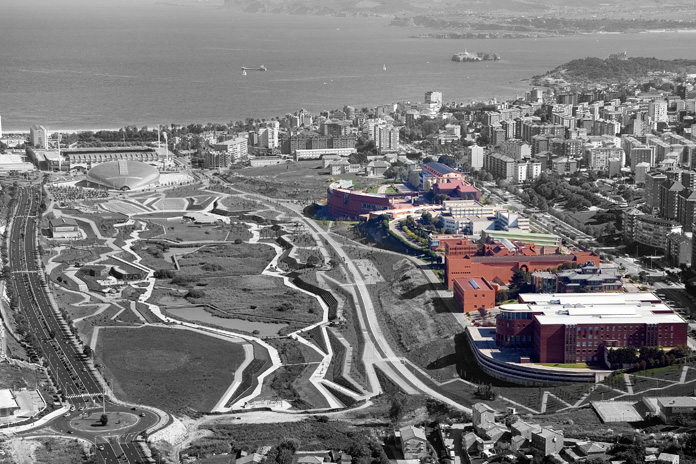
\includegraphics[width=\textwidth]{fig/Campus_las_llamas_3.jpg}
\end{center}
\caption{\label{fig:campusllamas}
Vista panorámica del Campus de Las Llamas de la Universidad de Cantabria, en Santander. Fuente: Adaptada de web.unican.es (Relaciones Internacionales, Galería de Fotos)}
\end{figure}

\paragraph{Reseña histórica de la Universidad de Cantabria\\\\}

La Universidad de Cantabria comenzó a fraguarse a principios del siglo XIX, a iniciativa de las entidades locales y provinciales de la región.  La Junta de Comercio asumió en 1829 la responsabilidad docente que hasta la fecha ejercía el Consulado del Mar, creando las Escuelas de Comercio y Náutica. Nueve años más tarde, el Ayuntamiento y la Diputación colaboraron para propiciar la creación del Instituto Cántabro de Enseñanza Media, que catalizaría los estudios que posteriormente cuajaron en las Escuelas de Grado Medio. Ya en el siglo XX, diversos centros docentes ascendieron de rango. En 1901 se creó la Escuela de Industrias; la Escuela Normal de Maestros inició su andadura en 1915; y en 1929 se fundó la Escuela de Enfermeras del Hospital Valdecilla. La implantación de nuevos centros continuó en la década de los cincuenta, periodo en el que Torrelavega acogió la Escuela de Magisterio de los Sagrados Corazones, la Escuela de Facultativos de Minas y Fábricas Minero-Metalúrgicas y Minero-Químicas y, en 1969, la Escuela de Graduado Social, dependiente de la Universidad de Oviedo.

La intervención de los poderes locales fue decisiva en la implantación en Santander de la Escuela Técnica Superior de Ingenieros de Caminos, Canales y Puertos (1966), una vez que el Ministerio hizo públicos sus planes de expansión de centros universitarios. Tres años más tarde inició su andadura la especialidad de Físicas de la Facultad de Ciencias, dependiente, junto con la Escuela de Caminos, de la Universidad de Valladolid. En 1971, el Ayuntamiento y la Diputación Provincial de Santander adquieren unos terrenos en el polígono de Las Llamas para la creación de un campus de 600.000 metros cuadrados (Figura \ref{fig:campusllamas}). Poco después, el III Plan de Desarrollo Económico Social, aprobado por Ley 22/1972 de 10 de mayo, dispuso el incremento y diversificación de los estudios superiores con la creación de nuevas universidades.  El 18 de Agosto de 1972, en virtud del Decreto 2566/1972, de 18 de agosto (BOE de 30 de septiembre), se creó la Universidad de Santander, germen de lo que, trece años más tarde, pasaría a denominarse Universidad de Cantabria.

\begin{table}[!ht]
\centering
\begin{tabular}{|l|}
\hline\hline
\multicolumn{1}{|c|}{\textbf{Centros Universitarios}}\\
\hline\hline
\textbf{Campus de las Llamas} \\
\hline 
Escuela Técnica Superior de Ingenieros de Caminos, Canales y Puertos\\
Facultad de Ciencias \\
Facultad de Filosofía y Letras \\
Facultad de Ciencias Económicas y Empresariales \\
Facultad de Derecho \\
Facultad de Educación \\
Escuela Técnica Superior de Ingenieros Industriales y de Telecomunicación \\
Escuela de Doctorado \\
\hline
\textbf{Campus de Torrelavega} \\
\hline 
Escuela Politécnica de Ingeniería de Minas y Energía \\
Escuela Universitaria de Fisioterapia Gimbernat-Cantabria \\
\hline
\textbf{Otros centros}\\
\hline
Escuela Técnica Superior de Naútica \\
Escuela Universitaria de Enfermería \\
Escuela Universitaria de Turismo Altamira\\
Facultad de Medicina \\
Centro Internacional de Estudios Superiores del Español\\
\hline\hline
\multicolumn{1}{|c|}{\textbf{Fundaciones e Institutos de Investigación}}\\
\hline\hline
Fundación Leonardo Torres Quevedo \\
Fundación Instituto de Hidráulica Ambiental de Cantabria \\
Fundación para el Estudio y la Investigación del Sector Financiero \\
Instituto de Física de Cantabria \\
Instituto de Hidraúlica Ambiental “IH Cantabria” \\
Instituto de Biomedicina y Biotecnología de Cantabria \\
Instituto Internacional de Investigaciones Prehistóricas de Cantabria \\
\hline\hline
\end{tabular}
\caption{\label{tab:centrosunican} Centros, fundaciones e institutos de investigación de la Universidad de Cantabria}
\end{table}

La Facultad de Medicina, que comenzó a impartir sus primeras clases en 1973, completó el número de centros establecidos por la Ley para la formación del distrito universitario.  En este mismo año, se inauguró el edificio de la Facultad de Ciencias y se aprobó la adscripción de las escuelas universitarias de Ingeniería Técnica Industrial, Empresariales, Ingeniería Técnica de Minas y Profesorado de EGB.  Durante los años siguientes se configuraron el resto de centros que componen hoy en día la Universidad de Cantabria (Tab. \ref{tab:centrosunican}).
 
Los estatutos de la Universidad de Cantabria se publicaron en el BOE en 1985. Al tiempo, los departamentos pasaron a convertirse en los órganos básicos para la docencia y la investigación. En 2003 se publicaron en el BOC unos nuevos Estatutos de la Universidad de Cantabria. Dicho texto legal pretendía dotar a la universidad de una herramienta útil para su integración de forma competitiva en el nuevo espacio de educación superior, tras la promulgación de la LOU de 2001. Posteriormente, con objeto de adaptarse a la ley 2/2011 de Economía Sostenible y a la ley 14/2011 de la Ciencia, la Tecnología, y la Innovación en Ciencia, así como a otras normas de rango inferior que desarrollan aspectos relevantes de la vida universitaria, tales como el Real Decreto 1393/2007, 29 de octubre, por el que se establece la ordenación de las enseñanzas universitarias oficiales; el Real Decreto 1791/2010, de 30 de diciembre,
por el que se aprueba el Estatuto del Estudiante Universitario; y el Real Decreto 99/2011, de 28 de enero, por el que se regulan las enseñanzas oficiales de doctorado; la Universidad de Cantabria elaboró unos nuevos estatutos que fueron aprobados en el Decreto 26/2012 del BOC.  
 
Aparte de los centros docentes, la UC cuenta actualmente con varias fundaciones e institutos para poner la investigación en diversas áreas del conocimiento al servicio de la sociedad. Entre los años 1980 y 1981 se aprobaron los Estatutos y la Carta Fundacional de la Fundación Leonardo Torres Quevedo, una iniciativa de la Escuela Técnica Superior de Ingenieros de Caminos, Canales y Puertos para promover la investigación en la misma, siendo reconocida y clasificada por el Ministerio de Educación y Ciencia e inscrita en el Registro Mercantil al año siguiente. En el año 1998 se modifican los estatutos y se incluyen entre sus objetivos el fomento y la promoción de la investigación en la Universidad de Cantabria y la formación de profesionales en las áreas científica y tecnológica.

En 1995 se constituyó el Instituto de Física de Cantabria (IFCA), centro mixto de la Universidad de Cantabria y el Consejo Superior de Investigaciones Científicas (CSIC) orientado a la investigación de los componentes de la naturaleza, desde las partículas elementales a las estructuras más grandes del Universo, así como el complejo comportamiento colectivo de la materia. Posteriormente el IFCA consolidó una nueva línea de investigación en Meteorología y Minería de Datos la cual conforma, junto con el Grupo de Meteorología y Computación de la Universidad de Cantabria, el Grupo de Meteorología de Santander.

La Fundación UCEIF para el Estudio y la Investigación del Sector Financiero, con el Banco Santander, comienza su andadura en 2006, con la misión de convertirse en un foro pionero y especializado para la generación y difusión del conocimiento, la formación, investigación y desarrollo dentro del ámbito financiero.

La Fundación Instituto de Hidráulica Ambiental de Cantabria echa a andar en 2007, constituida por representantes del Gobierno de Cantabria y la Universidad con el propósito de fomentar la investigación básica y aplicada y el desarrollo de estudios, metodologías y herramientas para la gestión integrada de los ecosistemas acuáticos. Para el desarrollo de tales fines, la Fundación Instituto de Hidráulica Ambiental de Cantabria y la Universidad de Cantabria crearon ese mismo año el Instituto de Hidráulica Ambiental de Cantabria (IH Cantabria), que aspira a ser referente internacional en su ámbito.
 
También en 2007 comienza a funcionar el Instituto de Biomedicina y Biotecnología de Cantabria (IBBTEC), a raíz de un convenio suscrito entre el Gobierno regional, el CSIC y la Universidad de Cantabria. El IBBTEC constituye el segundo centro mixto del CSIC en Cantabria y se concibe como un centro de investigación de excelencia en las áreas de biomedicina y biotecnología, impulsando la transferencia de resultados y tecnología a la sociedad y el sector productivo.

Estos institutos cuentan con infraestructuras punteras en el ámbito científico, destacando la participación del IFCA en la Red Española de Supercomputación con el supercomputador Altamira y la creación en el Instituto de Hidráulica Ambiental del Gran Tanque de Ingeniería Marítima, que es una Infraestructura Científico- Tecnológica Singular del Gobierno de España.

La Universidad de Cantabria es reconocida (desde 2009) como ``Campus de Excelencia Internacional CEI 2009 de ámbito regional'' gracias a su proyecto ``Cantabria Campus Internacional'', presentado junto con la Universidad Internacional Menéndez Pelayo (UIMP) con el apoyo de 16 instituciones representativas de la región. La UC fue una de las nueve universidades españolas seleccionadas en esta primera convocatoria del Ministerio de Educación, recibiendo tal calificación por su alto potencial para alcanzar el nivel de excelencia regional una vez se ponga en marcha el proyecto. Cantabria Campus Internacional, con sus seis áreas estratégicas (agua y energía; biomedicina y biotecnología; banca, finanzas y actividades empresariales; patrimonio y lengua; tecnología; y física y matemáticas) constituye un modelo de desarrollo de toda la sociedad cántabra basado en el conocimiento, en la innovación y en la sostenibilidad. 


\paragraph{Universidades europeas: la alianza EUNICE\\\\}

La Universidad de Cantabria fue seleccionada en la segunda convocatoria de ``Universidades europeas'' de la Comisión Europea, para formar parte del proyecto EUNICE (European University for Customised Education). La alianza está integrada por la Universidad tecnológica de Poznan (Polonia), coordinadora de la iniciativa; la Universidad de Cantabria; la Universidad de Mons (Bélgica); la Universidad politécnica Hauts-de-France (Francia); la Universidad de Vaasa (Finlandia); la Universidad técnica de Brandeburgo (Alemania) y la Universidad de Catania (Italia). Se trata de una alianza entre universidades de tamaño medio con perfiles complementarios, incluyendo miembros de perfil politécnico, de ciencias sociales y humanidades, o generalista, como es el caso de la UC. A través de la ``agregación'' ascendente de las siete universidades geográficamente equilibradas, EUNICE ofrecerá una educación personalizada, competitiva de clase mundial que satisfaga las necesidades de la sociedad, la vida laboral y el sector industrial e intercultural, pues fortalecerá la identidad europea y promoverá valores europeos comunes a través del interculturalismo, incluido el multilingüismo.

Esta iniciativa tendrá una importancia capital en los años venideros, requiriendo la adaptación de todo el profesorado, personal de administración y servicios y alumnado para acomodar este proyecto europeo que pretende dar forma a las universidades del futuro. 



\subsection{La Facultad de Ciencias}

La actual Facultad de Ciencias nació en 1969 en el seno de la Universidad de Valladolid, con la sección de Físicas como especialidad. Tres años después, la Facultad de Ciencias fue el germen de la Universidad de Santander junto a la Escuela Técnica Superior de Ingenieros de Caminos, Canales y Puertos y la recién creada Facultad de Medicina. En 1977 se implantó la sección de Matemáticas, completándose así la oferta académica a la que los alumnos pueden acceder desde
entonces. En todo este tiempo la Facultad se ha ido haciendo con una plantilla altamente competente de profesorado; entre éstos se cuentan académicos, premios de investigación, miembros de comisiones de expertos científicos a nivel internacional y otros profesionales de reconocido prestigio. En definitiva, la Facultad de Ciencias es uno de los centros más antiguos de la Universidad de Cantabria y presenta una inequívoca vocación de futuro. 

\paragraph{Estudios en la Facultad de Ciencias\\\\}

La Facultad de Ciencias de la Universidad de Cantabria imparte tres titulaciones de grado adaptadas al Espacio Europeo de Educación Superior (EEES) y siete titulaciones de máster oficial. Además se ha diseñado un itinerario de doble grado y se imparte un diploma durante el segundo cuatrimestre. La Facultad está también involucrada, desde el año 2014, en la impartición del programa de doctorado en Ciencia y Tecnología. Este programa procede de dos programas de doctorado con mención de excelencia. La Tab.~\ref{tab:estudios} resume la oferta académica ofrecida por la Facultad.

\begin{table}[!ht]
\centering
\begin{tabular}{|l|}
\hline\hline
\multicolumn{1}{|c|}{\textbf{Grado}}\\
\hline\hline
Grado en Física \\
Grado en Matemáticas \\
Grado en Ingeniería Informática \\
Doble Grado en Física y Matemáticas \\
International Diploma in Physics \\
\hline\hline
\multicolumn{1}{|c|}{\textbf{Máster}}\\
\hline\hline
Máster Universitario en Data Science \\
Máster Universitario en Ciencia e Ingeniería de la Luz \\
Máster Universitario en Física de Partículas y del Cosmos \\
Máster en Ingeniería Informática \\
Máster en Matemáticas y Computación \\
Máster Universitario en Nuevos Materiales \\
Máster Universitario en Química Teórica y Modelización Computacional \\
\hline\hline
\multicolumn{1}{|c|}{\textbf{Doctorado}}\\
\hline\hline
Doctorando en Ciencia y Tecnología \\
\hline\hline
\end{tabular}
\caption{\label{tab:estudios} Estudios de grado, máster y doctorado impartidos en la facultad de ciencias de la Universidad de Cantabria}
\end{table}

\paragraph{Estructura departamental de la Facultad de Ciencias\\\\}

La Facultad de Ciencias está organizada internamente en Departamentos. La Tab.~\ref{tab:departamentos} refleja los departamentos por áreas temáticas. Las actividades docentes en la Facultad tienen participación también de profesorado de Departamentos de otros centros de la Universidad. También es preciso mencionar al Instituto de Física de Cantabria (IFCA), centro mixto del Consejor Superior de Investigaciones Científicas y la Universidad de Cantabria. Muchos de los miembros del IFCA forman parte de la Facultad de Ciencias y contribuyen a las tareas docentes propias de ella.


\begin{table}[!ht]
\centering
\begin{tabular}{|l|}
\hline\hline
\multicolumn{1}{|c|}{\textbf{Física}}\\
\hline\hline
Departamento de Física Moderna \\
Departamento de Física Aplicada \\
Departamento de Ciencias de la Tierra y Física de la Materia Condensada  \\
\hline\hline
\multicolumn{1}{|c|}{\textbf{Matemáticas}}\\
\hline\hline
Departamento de Matemáticas, Estadística y Computación\\
\hline\hline
\multicolumn{1}{|c|}{\textbf{Ingeniería Informática}}\\
\hline\hline
Departamento de Ingeniería Informática y Electrónica \\
\hline\hline
\end{tabular}
\caption{\label{tab:departamentos} Departamentos de la Facultad de Ciencias de la Universidad de Cantabria}
\end{table}

\section{Docencia: criterios pedagógicos y metodológicos}
\label{metodologicos}

El compromiso de la Universidad con sus alumnos es el de proporcionarles una formación adecuada para que éstos puedan ejercer posteriormente, de forma responsable y eficaz, la labor profesional a la que accedan gracias a sus estudios. Este compromiso, especialmente en el caso de las titulaciones técnicas y científicas, no supone proporcionar un gran número de conocimientos altamente especializados, sino una formación general, amplia y rigurosa de todas las ciencias básicas que constituyen el armazón de la disciplina en cuestión. El objetivo principal de la labor docente debe ser formar al alumno en la materia correspondiente, con especial énfasis en el desarrollo de su capacidad y criterio personal, de manera que puedan aplicar los conocimientos básicos adquiridos en la solución de problemas técnicos y científicos y afrontar los nuevos cambios con total garantía. No es el contenido informativo de las teorías, sino la formación de un hábito reflexivo, lo que produce en definitiva una cultura científica.

La labor docente debe conseguir unos resultados a través de una adecuada planificación del curso, que ha de tener en cuenta el contenido de las materias a impartir (programa), los medios de los que se dispone y las actividades docentes a realizar. Existen una serie de objetivos generales que se pretenden alcanzar con la labor docente de una ciencia experimental, entre los que cabe destacar los siguientes~\cite{zabalza}:

\begin{enumerate}
\item	Conseguir la transmisión de conocimientos, técnicas y valores de una generación a otra, incorporando progresivamente aquellos avances y mejoras que se descubran, siempre con la finalidad de obtener una sociedad más justa e igualitaria en el sentido más amplio de progreso social.
\item	Facilitar la asimilación del método científico como procedimiento de abordar problemas y proyectos.
\item	Compaginar la visión científica (teórica) con la tecnológica (práctica), favoreciendo la interconexión de los conocimientos, procedimientos y técnicas básicas y su universalización.
\item	Aproximar al estudiante a la realidad de la empresa, industria, etc., integrándolo en la realidad socio-económica más próxima.
\item	Obtener y utilizar la información del área de conocimiento correspondiente, o de aquéllas relacionadas con la misma, de forma autónoma y crítica. Conocer la forma y los procedimientos de acceso a la información.
\item	Poseer autonomía para plantear cuestiones, elaborando y desarrollando estrategias de identificación de problemas, proponiendo alternativas y evaluando su actuación en la resolución de problemas, siguiendo un proceso de razonamiento lógico.
\item	Analizar, discutir y emitir valoraciones sobre el trabajo propio y ajeno.
\end{enumerate}

Siempre se tendrá en cuenta que además de las enseñanzas impartidas en un área concreta, se debe impartir de algún modo el camino de entendimiento que les capacite para el desarrollo de dichos conocimientos en un mundo interdisciplinar.

Las etapas en que se estructura el método didáctico son tres:
\begin{enumerate}
\item	Planificación de las enseñanzas a impartir o planificación docente.
\item	Comunicación de los conocimientos o práctica docente.
\item	Valoración del nivel de preparación alcanzado por el alumno y valoración de la labor docente, o evaluación.
\end{enumerate}


\subsection{Planificación y preparación docente} \label{sec:planificacion}

La selección del contenido que va a tener una asignatura es donde comienza la labor del profesor, que junto con la habilidad docente para transmitir esos conocimientos y la capacidad para estimular el interés de los alumnos, constituyen las piezas claves del proceso formativo.

Es evidente que para planificar con éxito la asignatura y, por tanto, elaborar un programa docente realista y equilibrado, es necesario elegir los conocimientos que se van a impartir y ordenarlos de manera lógica en función de los objetivos propuestos y el tiempo disponible. Ello exige un perfecto conocimiento de las materias que integran la disciplina y un amplio panorama del contexto en el que se engloba. Sólo de esta forma puede distinguirse entre lo fundamental y lo secundario, y así poder proporcionar una visión lo más completa posible de la asignatura en el tiempo, normalmente insuficiente para un desarrollo amplio, del que se dispone. Esta limitación temporal es inevitable; por ello, debe evitarse un enfoque excesivamente aislado de los temas, centrándose en métodos y aspectos comunes y en la relación existente con otras disciplinas. Esto permitirá al alumno profundizar por su cuenta en aquellos temas de su interés.

Otro aspecto fundamental a analizar a la hora de establecer los objetivos que se desea lograr en el desarrollo de una asignatura es la situación de ésta en el contexto global de la carrera. Se trata de tener en cuenta la formación previa del alumno y la que pueda adquirir en cursos posteriores; de esta manera se facilitará el aprendizaje, a la vez que lo aprendido se convertirá en una base sólida para la comprensión de nuevos conceptos en otros cursos.

\subsection{Práctica docente} \label{sec:practica_docente}

La etapa de comunicación de los conocimientos representa la etapa más atrayente en la actividad docente. En esta etapa se pretende no sólo enseñar los fundamentos y métodos característicos de la disciplina, sino también procurar que el alumno los utilice, ayudándole a descubrir y plantear sus problemas, a diseñar experimentos, a encontrar respuestas aportando datos, dando pistas, etc., y también a alcanzar cada vez mayor rigor y a realizar su trabajo de forma sistemática.

La tradicional división entre clases teóricas y clases prácticas, y dentro de estas últimas, sus variantes de laboratorio, problemas y seminario, obedecen, probablemente, más a la forma que al fondo. Unas y otras tienen la misma misión, conseguir la comunicación de unos mismos conocimientos, diferenciándose fundamentalmente en la forma en que éstos se transmiten. Si estas clases se imparten por distintos profesores y si, además, su contenido no responde a la necesaria unidad, se pueden provocar unas divisiones carentes de fundamento.


\paragraph{Clases teóricas\\\\}

Las clases de teoría o clases magistrales son el núcleo fundamental de desarrollo del programa de la asignatura. Es la forma más tradicional de enseñanza universitaria. Su origen reside en las épocas en que la comunicación verbal era claramente más asequible que la comunicación escrita, pero ha conservado su preponderancia porque además permite una flexibilización en el contenido, tanto extensivo como intensivo, incorporando el diálogo de profesores y alumnos. Aunque el método presenta ventajas que hacen difícil prescindir de él, ha sido también ampliamente criticado.  Estudios recientes muestran que inmediatamente después de una clase los alumnos recuerdan el 70\% de la información presentada en los diez primeros minutos y sólo el 20\% de lo expuesto en los diez últimos minutos.

Para impartir las clases teóricas, pueden tomarse como base las directrices dadas por el Instituto de Ciencias de la Educación (ICE) de la Universidad Politécnica de Madrid para el perfil de una lección ideal, que se expone a continuación:

\textbf{Motivación}
\begin{enumerate}
\item Motivar antes y durante la clase para que el alumno se interese por la asignatura. Esto requiere:
\begin{itemize}
\item Que el profesor muestre entusiasmo por la asignatura.
\item Que el profesor demuestre seguridad científica.
\end{itemize}
\item Conectar con la realidad. El profesor debe mostrar los aspectos reales del tema, así como las consecuencias prácticas. Para ello es necesario: centrar el tema con un ligero bosquejo histórico, citar las tecnologías en que será útil, explicar las consecuencias prácticas, citar ejemplos de aplicación, etc.
\end{enumerate}

\textbf{Aspectos del contenido}
\begin{enumerate}
\item Introducción al tema. Presentación de los objetivos y contenidos de la lección. Esto requiere:
\begin{itemize}
\item Resumir los objetivos didácticos.
\item Anunciar el desarrollo del tema.
\item Resumir los conocimientos previos que se necesitan.
\end{itemize}
\item Ordenación del tema. El desarrollo ordenado y sistemático del tema precisa:
\begin{itemize}
\item Presentar un resumen del tema por escrito.
\item Evitar saltos hacia atrás o laterales en la explicación.
\item Reforzar los conceptos básicos cuando aparezcan.
\end{itemize}
\item Síntesis y/o recapitulaciones. Esfuerzo para que el alumno consolide los conocimientos adquiridos y los integre. Para ello es necesario:
\begin{itemize}
\item Repetir los puntos fundamentales del tema.
\item Establecer lazos con las partes pasadas y futuras de la asignatura.
\end{itemize}
\end{enumerate}

\textbf{Aspectos formales de la comunicación}
\begin{enumerate}
\item Claridad de expresión. Habilidad para transmitir el mensaje didáctico mediante:
\begin{itemize}
\item Utilización correcta del lenguaje.
\item Buena dicción.
\item Uso de pausas.
\item Uso de gestos, etc.
\end{itemize}
\item Recursos didácticos. Uso de toda clase de medios físicos para reforzar y/o aclarar el mensaje. Esto requiere:
\begin{itemize}
\item Uso de medios audiovisuales.
\item Reparto de documentación complementaria.
\item Dibujo directo de esquemas, ejemplos,...
\end{itemize}
\end{enumerate}

\textbf{Organización y animación de la clase}
\begin{enumerate}
\item Participación de los alumnos en la construcción de los conceptos y petición por su parte de las aclaraciones oportunas. Ello conlleva:
\begin{itemize}
\item Información previa a los alumnos de que sus intervenciones serán bien acogidas.
\item Realización de preguntas adecuadas.
\item Refuerzo y ponderación de todas las contestaciones acertadas.
\item Explicación afable de las contestaciones no acertadas.
\end{itemize}
\end{enumerate}

\textbf{Control}
\begin{enumerate}
\item Control permanente del grado de atención y asimilación del alumno. Para ello se necesita:
\begin{itemize}
\item Vigilancia del grado de atención de los alumnos a través de sus gestos.
\item Atención a las condiciones de los alumnos.
\item Realización de preguntas tipo test.
\item Utilización de técnicas objetivas de control.
\end{itemize}
\end{enumerate}


\paragraph{Clases de problemas\\\\}

Las clases de problemas cumplirán con la función de complementar las clases de teoría y hacer más fácil su comprensión, así como de captar los puntos del mecanismo de razonamiento de la materia que causan más dificultades de comprensión a los alumnos. Por ello, es fundamental simultanear las clases de teoría con las correspondientes de problemas que ayuden a fijar los conocimientos adquiridos.


Las cuestiones o problemas propuestos se deben seleccionar cuidadosamente, para que posean dos características fundamentales: en primer lugar han de servir para aplicar los conocimientos desarrollados en las clases teóricas precedentes, y en este sentido será necesario para su resolución utilizar las gráficas, tablas etc. que se hayan estudiado con anterioridad; en segundo lugar, deben reflejar situaciones reales siempre que sea posible, lo que llevará consigo la discusión de los resultados obtenidos, y en ocasiones comentarios sobre el procedimiento de resolución que se haya seguido.

Respecto a la resolución de problemas en clase, debe seguirse un esquema lógico: planteamiento del problema, esquema de resolución más adecuado, discusión de los resultados obtenidos y su aplicación a la realidad. No es conveniente que el profesor resuelva siempre los problemas íntegramente en la pizarra sin la participación del alumno. Resulta más adecuado que el estudiante resuelva los problemas después de que el profesor haya esbozado someramente el método para su resolución. Así, la clase de problemas supone una participación activa del alumno en la discusión de las dudas que hayan podido presentarse. Para conseguir esto, hay que distribuir los enunciados con suficiente antelación para que los alumnos puedan resolverlos. También se puede establecer algún incentivo, como tener en cuenta en la evaluación global el hecho de que los alumnos entreguen los  problemas previamente resueltos, o incluso, si la colección de problemas fuese lo suficientemente grande, indicarles que algún problema semejante a los que se les ha repartido, formará parte de la evaluación escrita.


\paragraph{Seminarios\\\\}

Cuando es posible trabajar con grupos reducidos de alumnos, se puede recurrir a las clases de seminario, que deben ser lo suficientemente flexibles para que, en primer lugar, subsanen las deficiencias que se detecten en las clases teóricas y de problemas. En estas últimas, donde el alumno toma contacto por primera vez con muchos temas, es muy difícil que pueda establecerse un diálogo fructífero o una captación satisfactoria de las enseñanzas. Además y de acuerdo con el plan seguido, existirán algunos aspectos, o conocimientos, cuyas características peculiares no aconsejen abordarlos en las clases teóricas.

Además de estos objetivos de reforzar los conocimientos de base del alumno, que le faciliten el normal aprendizaje de las asignaturas, los seminarios pueden cubrir un segundo objetivo, el de ampliar los conocimientos impartidos en las clases de teoría. En este sentido, los seminarios proporcionan una buena ocasión para incidir en la importancia de la consulta de fuentes bibliográficas, introduciendo al alumno en el uso y manejo de redes automatizadas.


\paragraph{Prácticas en el laboratorio o en el aula de informática\\\\} \label{sec:practicas}

El aprendizaje de materias tecnológicas y de carácter aplicado exige la experiencia directa con sistemas y elementos reales, que permita la comprensión práctica de los conocimientos adquiridos en las clases de teoría y problemas y la aplicación de los mismos a la resolución de problemas reales. La práctica desarrolla la capacidad de observación y toma de decisiones y asegura el contacto con la realidad profesional. Muchos de estos objetivos pueden conseguirse también a través del uso de ordenadores, bien para elaborar prácticas que requieran cálculos complejos, o bien para utilizar simuladores que permitan profundizar en los conceptos explicados en las clases de teoría.

El objetivo de las clases prácticas en laboratorio puede concretarse en dos puntos:
\begin{enumerate}
\item	Las prácticas deben mostrar cómo los principios tratados en las clases teóricas y de problemas se aplican al diseño, realización y comprobación del sistema físico y/o su modelo informático. Deben realizarse experiencias concretas que ayuden a los estudiantes a comprender los conceptos abstractos. Estas experiencias son esenciales para agudizar la intuición de los alumnos en temas prácticos, y para poner de relieve el esfuerzo intelectual necesario para la construcción de modelos analíticos de sistemas reales.
\item	Deben destacar el desarrollo de las actividades específicamente proyectuales y en la utilización de metodologías generales, evitando una concreción excesiva provocada por la tipología concreta del problema.
\end{enumerate}

La temática de las prácticas debe basarse en los conceptos que están siendo estudiados en teoría en cada momento. Así, el alumno podrá aplicar los conocimientos recién adquiridos, obteniendo el mayor aprovechamiento posible. Para conseguir un máximo aprovechamiento de este tipo de enseñanza es conveniente que los trabajos se efectúen en grupos reducidos. La realización de unas prácticas útiles y sugestivas es un elemento motivador, que crea en el alumno interés, incluso la necesidad de adquirir la teoría correspondiente.

Un desarrollo correcto de las sesiones prácticas debe seguir los pasos que se enumeran a continuación:
\begin{enumerate}
\item	Especificar los objetivos de la práctica.
\item	Descripción del material a utilizar.
\item	Descripción del trabajo a desarrollar.
\item	Desarrollo de la actividad propuesta.
\item	Indicaciones sobre la redacción de la memoria de la práctica y los resultados a presentar.
\end{enumerate}


\paragraph{Acceso a las nuevas tecnologías y Aula Virtual\\\\} \label{sec:aulavirt}

La integración de las redes telemáticas en la educación ha provocado, en pocos años, importantes modificaciones en la naturaleza y procesos de enseñanza, en las formas y sistemas de comunicación y relación entre alumnos y profesores, así como en las modalidades educativas que se ofertan desde las universidades~\cite{duder97,pimentel99,reid99}. En este marco cobra sentido la necesidad de organizar institucionalmente un nuevo espacio para la docencia apoyado en el uso de las redes de comunicación digitales. Este nuevo escenario para la docencia distribuida a través de Internet se conoce como Campus Virtual. Un campus virtual, en consecuencia, es la respuesta universitaria al reto de integrar las nuevas tecnologías con la finalidad de extender la oferta docente a nuevos colectivos de ciudadanos para que cursen los estudios a distancia, a la vez, que puede servir para innovar y mejorar los métodos tradicionales de enseñanza en la universidad.

Internet permite el desarrollo de variadas actividades de enseñanza utilizando los recursos telemáticos (WWW, e-mail, chat, videoconferencia, $\ldots$). Cuando estas acciones educativas están organizadas institucionalmente por una universidad y distribuidas a través de redes de ordenadores podemos hablar de un \textbf{\emph{campus virtual}}. Un campus virtual, en consecuencia, se podría definir como un espacio formativo ofertado por una institución universitaria que se desarrolla a través de redes digitales.

Este espacio educativo virtual puede servir para el desarrollo de dos grandes funciones pedagógicas~\cite{area01}:

\begin{enumerate}
\item	La red como apoyo a la docencia presencial. El campus virtual puede ofertar, a través de la red, materiales y recursos didácticos de apoyo a la docencia universitaria presencial. Esta función sirve para facilitar la integración y uso de las nuevas tecnologías (multimedia, tutoriales web, chats educativos, videoconferencia, $\ldots$), en las clases convencionales de modo que se complementen las actividades formativas presenciales con otras realizadas en la red. La existencia de un 'campus virtual' en las universidades convencionales hace posible que el profesorado pueda diseñar y publicar sus materiales didácticos de estudio de la asignatura, que permita la realización de actividades en la red como debates telemáticos entre el alumnado; las consultas y tutorías electrónicas. En consecuencia un 'campus virtual' debe entenderse, al menos en las universidades convencionales, como complemento de su actividad y organización docente.
\item	La red como escenario para la educación a distancia. El campus virtual también puede servir para ofertar una modalidad de enseñanza a distancia o teleformación de los estudios universitarios (tanto los de las titulaciones de primer y segundo ciclo, como de cursos de postgrado) a través de las redes digitales. Con ello se persigue extender la oferta de enseñanza superior a más grupos de ciudadanos de los que actualmente cursan sus estudios en las aulas convencionales de cada universidad. Esta segunda modalidad o función del campus virtual abre la posibilidad de cursar los estudios de enseñanza superior desde su hogar o lugar de trabajo a aquellos colectivos sociales que por motivos de edad, situación profesional o residencia no acuden a las aulas.
\end{enumerate}

Un aula virtual es un entorno, plataforma o software a través del cual el ordenador simula una clase real permitiendo el desarrollo de las actividades de enseñanza y aprendizaje habituales. Como afirma Turoff~\cite{turoff95} una \emph{'clase virtual es un entorno de enseñanza y aprendizaje inserto en un sistema de comunicación mediado por ordenador'}. A través de ese entorno el alumno puede acceder y desarrollar una serie de acciones que son las propias de un proceso de enseñanza presencial como conversar, leer documentos, realizar ejercicios, formular preguntas al docente, trabajar en equipo, etc. Todo ello de forma simulada sin que medie una interacción física entre docentes y discentes. En estos momentos existen en el mercado numeroso software que permite la creación de cursos a distancia simulando aulas virtuales como por ejemplo \texttt{Learning Space}, \texttt{WebCT}, \texttt{eCollege}, \texttt{Aula Virtual}, \texttt{Moodle}, etc.

En consecuencia, la creación, mantenimiento y desarrollo de programas y cursos ofertados virtualmente debe ser planteado como una estrategia de mejora educativa que movilice distintos recursos técnicos y humanos de cara a ampliar el número de estudiantes de dicha universidad, así como para que su profesorado se implique en procesos de innovación de los métodos de enseñanza que utiliza.


\paragraph{Tutorías\\\\} \label{sec:tutor}

El sistema tutorial, introducido inicialmente en las universidades británicas, se basa en la asistencia individualizada que un profesor, denominado tutor, presta a un alumno o pequeño grupo de alumnos que le han sido asignados. Las tutorías ejercidas sobre los alumnos tienen una significación bien distinta a la del sistema tutorial inglés, puesto que en la práctica se reducen a proporcionar al estudiante una información general, si es que éste lo requiere, y ayudar a la resolución de sus dudas o cuestiones sobre la asignatura, que es el caso que más frecuentemente se demanda. En este sentido, es más importante potenciar la autonomía de los razonamientos del alumno que ofrecer soluciones inmediatas a las dificultades que se plantee en su proceso de aprendizaje. Por ello, situar y fundamentar la dificultad de adquisición de datos y conocimientos científico-técnicos, es uno de los objetivos prioritarios para las tutorías.


\paragraph{Otras actividades\\\\}

La organización de conferencias y debates impartidas por profesionales de ejercicio libre, expertos o profesores e investigadores de otros centros suele resultar muy interesante de cara al alumnado, ya que le permite tener una visión general de otros posibles planteamientos y alternativas, de problemáticas científicas y casos reales, etc. Igualmente le permite no atenerse únicamente al temario concreto de la asignatura. Adicionalmente, presenta la posibilidad de abrir contactos iniciales con investigadores, empresas y centros que trabajen sobre temas en los que el alumno tenga especial interés. 

Existen además nuevos conceptos pedagógicos como el ``Flipped Classroom'' o clase invertida~\cite{flipped} en el que la fase de transmisión de conocimientos, tradicionalmente centrada en la clase magistral, es trasladada al espacio de trabajo personal del estudiante, siendo sustituida por actividades que fomentan el refuerzo del aprendizaje y la adquisición de competencias. La aplicación de este método conlleva normalmente la ampliación de los recursos educativos ofrecidos al estudiante en forma de vídeos, textos adicionales, artículos de investigación, etc., de modo que se facilite el proceso de adquisición del conocimiento. De la misma forma, el método requiere también el diseño de una actividad presencial que desarrolle los conocimientos adquiridos por los estudiantes. Algunas opciones típicas tienen que ver con el planteamiento de actividades en equipo, o con la aplicación de conceptos de ``gamificación'' en la que los alumnos participan en juegos en los que necesariamente han de aplicar los conocimientos adquiridos. 

Los conceptos anteriores pueden beneficiarse también de herramientas online que facilitan la creación de cuestionarios en tiempo real, participación en equipo, o incluso plataformas que permiten realizar actividades de competencia lúdica entre los estudiantes. Algunos de los más populares son: Kahoot, Quizzit o Space Race. 



\paragraph{Trabajos de fin de grado\\\\} \label{sec:proyecto}

Para la obtención del título en las carreras técnicas, el alumno debe realizar un trabajo supervisado por un profesor de la Escuela, en la Universidad o en una institución pública o privada. La realización del Trabajo de Fin de Grado (TFG) permite al alumno profundizar en la metodología y morfología proyectuales a la vez que desarrolla un tema de su interés. Entre las opciones destacan trabajos originales de investigación científica, que serán algo más ambiciosos que un problema extenso, ya que exigirá una capacidad de análisis y síntesis mayor que la resolución de un simple problema. El alumno necesitará buscar datos, tendrá que tomar decisiones, relacionar varias asignaturas, diseñar elementos auxiliares, etc. El uso del ordenador, tanto para situaciones de diseño de operaciones mediante simuladores, como a la hora de realizar una optimización económica del proyecto, es altamente recomendado. Esta actividad, además de permitir contrastar lo aprendido con la realidad práctica, ejercita al máximo la capacidad creadora del alumno y constituye una fuente de temas de interés para el profesor.


\paragraph{Estudios de Máster\\\\}

El Espacio Europeo de Educación Superior establece los estudios de Máster como el primer nivel de especialización tras el desarrollo de los estudios de grado. Los estudios de Máster en España vienen regulados por el Real Decreto 1393/2007 por el que se establece la ordenación de las enseñanzas universitarias oficiales. La tipología de actividades docentes desplagadas en los estudios de Máster está contenida en el documento de ``Manual de procedimiento para la emisión del informe de evaluación de las solicitudes de implantación de títulos oficiales de posgrado'' elaborado por la ANECA, agrupando las actividades en dos grandes grupos: presenciales y no presenciales. Las primeras incluyen clases teóricas y seminarios, clases prácticas y actividades de dirección, seguimiento y evaluación: prácticas externas (en instituciones o empresas), tutorías o sesiones de evaluación. Las segundas a su vez incluyen el trabajo autónomo y el trabajo en grupo. Los estudios de Máster culminan con un Trabajo de Fin de Máster (TFM), que consistirá en la realización por parte del estudiante de un trabajo original, autónomo y personal, bajo la orientación de un profesor, en el que se apliquen y desarrollen los conocimientos y capacidades adquiridos a lo largo de la titulación, demostrando que ha alcanzado las competencias previstas en el plan de estudios.

\paragraph{Estudios de doctorado\\\\}

Además de la docencia en el grado, dentro de la labor del profesor universitario se incluye la formación de doctores y especialistas en distintas materias. Para la obtención del título de Doctor es necesario superar las pruebas de un programa de doctorado, que consisten en una serie de cursos de doctorado y la presentación de un trabajo original como tesis doctoral. Los estudios de doctorado quedan regulados por el real decreto 98/2011 y por su última modificación 195/2016. Los programas de doctorado incluyen aspectos organizados de formación investigadora que no requieren estructuración en créditos ECTS y comprenden tanto formación transversal como específica del ámbito de cada programa, si bien en todo caso la actividad esencial del doctorando es la investigadora. Los estudios de doctorado deben garantizar la adquisición de las siguientes competencias básicas:

\begin{itemize}
    \item Comprensión sistemática de un campo de estudio y dominio de las habilidades y
métodos de investigación relacionados con dicho campo.
\item Capacidad de concebir, diseñar o crear, poner en práctica y adoptar un proceso
sustancial de investigación o creación.
\item Capacidad para contribuir a la ampliación de las fronteras del conocimiento a través
de una investigación original.
\item Capacidad de realizar un análisis crítico y de evaluación y síntesis de ideas nuevas y
complejas.
\item Capacidad de comunicación con la comunidad académica y científica y con la sociedad en general acerca de sus ámbitos de conocimiento en los modos e idiomas de uso habitual en su comunidad científica internacional.
\item Capacidad de fomentar, en contextos académicos y profesionales, el avance científico,
tecnológico, social, artístico o cultural dentro de una sociedad basada en el conocimiento
\end{itemize}

La actividad docente en el caso de los programas de doctorado se condensa en la figura del director de la tesis doctoral, que será el máximo responsable de la coherencia e idoneidad de las actividades de formación, del impacto y novedad en su campo de la temática de la tesis doctoral y de la guía en la planificación y su adecuación, en su caso, a la de otros proyectos y actividades donde se inscriba el doctorando. 


\subsection{Evaluación de la docencia} \label{sec:evaluadoc}

\paragraph{Evaluación del aprendizaje del alumno\\\\} \label{sec:evaluacion_alumno}

Dado que el objetivo final de la enseñanza universitaria es la formación de profesionales capacitados para desarrollar una actividad profesional, es lógico que la sociedad exija que esos futuros profesionales estén capacitados para desempeñar ese trabajo. Por ello será necesario un procedimiento de valoración para conocer si han alcanzado el grado de capacitación adecuado.

La evaluación continuada, las pruebas, ejercicios o exámenes, constituyen los instrumentos que se utilizan en esta fase de valoración y que, manejados con habilidad, potencian la asimilación y fijación de las enseñanzas impartidas. Aunque existan muchos modos eficaces de utilizarlas, es difícil encontrar alguno que satisfaga todos los requisitos que, en principio, serían deseables, sobre todo cuando los cursos son numerosos y el tiempo de corrección limitado.

En cualquier caso, el criterio de valoración debe conseguir una preponderancia de los aspectos positivos sobre los negativos. Entre los primeros pueden enumerarse los siguientes como más importantes:
\begin{itemize}
\item	Ayudar al alumno a realizar su trabajo personal, siempre que las orientaciones de las clases se reflejen en las pruebas o controles que se realicen. Así, si en unas se consideran inútiles los esfuerzos memorísticos, en las otras no deben formularse aquellas cuestiones que los requieran. Si se insiste en la necesidad de un trabajo continuado, deben arbitrarse los medios que lo pongan de manifiesto. Por la misma razón, deben recibir una atención especial aquellos temas o conceptos que se hayan señalado como fundamentales, aunque sin olvidar los restantes. En caso contrario, se corre el peligro de desdibujar la formación del alumno, fomentando la preparación exclusivamente con vistas a lograr la superación de un examen, en lugar de un aprendizaje gradual y continuado.
\item	Sirven tanto al profesor como al alumno, para conocer los puntos o facetas que no han sido convenientemente asimilados y que por lo tanto, deben ser analizados o estudiados de nuevo.
\item	Además, los ejercicios deben ser consecuentes con el contenido y nivel de las explicaciones recibidas, evitando que su preparación o realización vaya en detrimento de ésta o de otras enseñanzas.
\end{itemize}

De acuerdo con lo expuesto anteriormente, parece inaceptable basar un método de valoración en un sólo examen de final de curso, cuya validez, incluso como termómetro de la materia asimilada, puede ser cuestionable. Las bases en las que asentar la valoración de conocimientos, en su doble finalidad de instrumento de medida y aprendizaje, podrían ser las siguientes:
\begin{itemize}
\item	Resolución de problemas semanalmente en horas no lectivas, de modo que el alumno disponga de las fuentes de información, consultas y tiempo que estime necesario. Si bien puede parecer que este tipo de prueba no aporta un dato fidedigno, puesto que en principio se presta a que tan sólo una parte de los alumnos resuelvan las cuestiones y el resto se limite a transcribirlas con su nombre, la experiencia ha demostrado que después de los primeros ejercicios, tan sólo aquellos que los resuelven, los presentan, mientras que los que en principio los transcribían, abandonan esta postura por considerarla inútil. Es indudable que esta prueba, por sí sola, es insuficiente para valorar al alumno, puesto que si éste conociera que es el único criterio de calificación, sacrificaría el esfuerzo personal en aras de una futura calificación. La finalidad positiva de este tipo de pruebas es que obligan al alumno, que cursa normalmente la disciplina, a un esfuerzo continuado, consciente de que su trabajo es valorado por el profesor.
\item	Discusión individual en clase de laboratorio. La realización de las prácticas, sobre todo si es posterior y acorde con las enseñanzas teóricas, permite, mediante preguntas adecuadas, conocer el esfuerzo realizado y la asimilación conseguida. Como parte positiva destaca la motivación del alumno para estudiar continuamente la teoría, y la oportunidad de enfocar adecuadamente su estudio, corrigiendo aquellos conceptos equivocados. El profesor debe hacer que el alumno conozca una técnica, sus aplicaciones y sus limitaciones.

\item	La formulación de cuestiones en clases de teoría, problemas o seminarios, impide valorar el nivel de cada alumno, si la clase como normalmente ocurre, es numerosa. Sin embargo, el profesor puede sacar conclusiones importantes sobre el grado de asimilación y sobre el modo en que se siguen sus enseñanzas.

\item	Realización de ejercicios o exámenes periódicos. El número de pruebas a realizar está sujeto a muchos condicionantes, pero puede considerarse como razonable una cada dos meses. Se considera totalmente necesario que el planteamiento de estos ejercicios vaya encaminado a desterrar los esfuerzos de última hora, que además de su poca utilidad, implican una discontinuidad en el trabajo del alumno. Para ello, las preguntas formuladas serán concretas, abarcarán siempre la totalidad de materia y versarán sobre aplicaciones conceptuales, unas cualitativas y otras cuantitativas, aspectos críticos y comparativos. Una vez corregido un ejercicio, conviene dedicar una clase a su comentario, resaltando los errores más importantes y explicando detalladamente el significado y solución de cada una de las cuestiones. La información conseguida sobre los conocimientos adquiridos y la formación alcanzada, por cada uno de los alumnos, debe ser analizada y, posteriormente, traducida en la calificación final.
\end{itemize}

\paragraph{Evaluación del profesor por parte del alumno\\\\}

La valoración por parte de los alumnos de la calidad de la enseñanza recibida es fundamental para que el profesor obtenga conclusiones sobre la marcha del curso. Esta información le permitirá revisar y reelaborar el programa de contenidos de acuerdo con las modificaciones necesarias para mejorar los resultados. Es fundamental que el profesor recabe el máximo de información sin temor a críticas, ya que de esta forma logrará corregir posibles errores en su planteamiento.

Esto puede abordarse en los cursos no muy numerosos a través del diálogo directo. Por razones obvias, en los cursos con mayor número de alumnos este diálogo se ve muy dificultado, por lo que la utilización de encuestas es recomendable, dado que éstas suministran una información objetiva y son libres dado su carácter anónimo.

El contenido de la encuesta debe centrarse en tres aspectos:
\begin{itemize}
\item Comportamiento personal, que se puede enfocar en preguntas sobre la actitud, accesibilidad, trato, puntualidad, etc., del profesor.
\item Planificación docente, que se puede enfocar con preguntas sobre dificultades de comprensión, orden en la exposición, etc.
\item Calidad e interés de la materia, que se puede enfocar con preguntas sobre la relación con otras asignaturas, etc.
\end{itemize}
La evaluación de estas encuestas debe fortalecer la reflexión sobre las actividades docentes y estar integrada en los mecanismos de control sobre la actividad del profesorado de cada Universidad.


\subsection{Recursos didácticos y tecnológicos para la docencia} \label{sec:recursos}

La mayoría de los profesores proporcionan a sus alumnos una lista de libros que pueden servir como base del aprendizaje o bien como apoyo. El profesorado que quiera mejorar su actividad docente tiene a su disposición, además de los recursos clásicos de la docencia universitaria, una serie de recursos tecnológicos audiovisuales e informáticos que le permitirán realizar innovaciones para incrementar el interés y la motivación del alumnado.

El profesor que escoge la presentación o clase magistral, dispone, además de los libros de texto y de consulta, de una serie de recursos que le ayudarán en su tarea. A continuación se presentan los recursos didácticos y tecnológicos.

\paragraph{Libros\\\\}

Prácticamente todos los profesores están de acuerdo en que, al comienzo del curso, debe proporcionarse al alumno bibliografía completa y actualizada sobre la materia a tratar lo más adecuada posible. La bibliografía a presentar en el programa de la asignatura debe contener los libros que sean realmente un recurso didáctico para el alumno, y asegurarse de la disponibilidad de estos libros en las bibliotecas y librerías. Un ejemplo de bibliografía útil para el alumno sería aquella que incluyera lo siguiente:
\begin{itemize}
\item	Referencias fundamentales: son los libros de lecturas necesarias y que podrían considerarse como los libros de texto del curso. Hay que procurar no especificar un único libro de texto, para que el alumno no dependa de un solo documento o autor. Asimismo, puede ser conveniente preparar dos o tres referencias fundamentales para cada capítulo o tema, para que el alumno haga un mejor uso de la bibliografía. Otra condición indispensable para sugerir un libro como referencia fundamental es que este sea de fácil acceso (en la biblioteca y en librerías conocidas). También conviene que la lista de referencias no sea muy extensa, para facilitar al alumno el acceso a la información fundamental. Además de libros de texto, sería muy conveniente para la mayoría de las asignaturas de física, el proporcionar una colección de problemas, global o por capítulos y de antemano, a fin de que el alumno pueda ir resolviéndolos y trabajando en la materia.
\item	Referencias básicas: incluirían las referencias necesarias para una formación completa en la materia, dentro de la línea o con la interpretación que el profesor considere adecuada. Estaría dirigida a alumnos que quisieran tener una visión completa de la asignatura.
\item	Referencias complementarias y de ampliación: aquí se puede incluir una extensa lista de libros, artículos y material escrito que puedan aportar informaciones relevantes en el ámbito de la asignatura o de algún tema concreto tratado, y que permitan al alumno profundizar más en la materia.
\end{itemize}

\paragraph{Recursos de soporte a la presentación oral\\\\}

\textbf{La pizarra}

La pizarra es el elemento soporte más utilizado para el desarrollo normal de las clases. Aunque tanto profesores como alumnos están muy habituados al uso de la pizarra, es importante hacer un uso correcto de ella. A continuación se presentan una serie de consejos prácticos para la utilización de la pizarra como soporte docente. Algunos consejos para la buena utilización de la pizarra son:
\begin{itemize}
\item	Escribir al lado de la pizarra al principio de clase un índice esquemático con los contenidos de la clase.
\item	Escribir siempre en la pizarra las palabras de grafía desconocida o que tengan que ser recordadas por los alumnos: términos científicos, referencias, expresiones numéricas, fórmulas, etc.
\item	Evitar textos largos.
\item	Distribuir el espacio físico de la pizarra convenientemente.
\item	Utilizar el color con moderación, y con alguna clave sencilla (por ejemplo, conceptos en blanco, ejemplos en azul, observaciones en verde, ...).
\item	Cuando sea importante que los alumnos conserven por escrito y con fidelidad la información de la pizarra, conviene repartirla por escrito.
\end{itemize}


\textbf{Presentaciones con ordenador}

El ordenador puede ser utilizado durante las clases don dos finalidades principales: 

\begin{enumerate}
\item Para ayudar al profesor en su explicación a través de presentaciones con transparencias en las que se muestran los contenidos de la asignatura incluyendo un soporte visual para mostrar gráficas, fotografías, etc.
\item Para mostrar contenidos multimedia que incluyan vídeos, simulaciones o demostraciones informáticas relacionadas con la asignatura. 
\end{enumerate}

El uso de presentaciones de ordenador requiere atención en dos aspectos fundamentales: el diseño de las transparencias y la parte activa del uso de la transparencia en la clase. Desde el punto de vista del diseño, las transparencias han de resultar claras y no estar excesivamente sobrecargadas de texto que distraiga del discurso principal del profesor. Normalmente es interesante desde un punto de vista pedagógico, asociar a cada transparencia un único concepto principal. El uso de índices o referencias interpuestas que ayuden a relacionar los conceptos entre sí y a enmarcarlos en el contexto global de la asignatura, es también beneficioso. Por otro lado, el uso de la transparencia ha de ser cuidadoso, manteniendo los tiempos que permitan al alumnado comprender sus contenidos. El uso de punteros para enfocar y dirigir la atención del alumno por la transparencia facilita también la comprensión global de los conceptos.  

\paragraph{Acceso telemático\\\\}

El uso de Internet se ha extendido ampliamente, no sólo en nuestro país. La red de Internet es una red mundial que, si bien a mitad de los años 80 apenas tenía unos miles de usuarios, en la actualidad se ha convertido en la red de comunicaciones más extendida. Algunas de las posibilidades que presentan al acceder a una red son:

\begin{itemize}
\item	Acceder a los archivos de bibliotecas de todo el mundo.
\item	Acceder a los archivos de biblioteca de la propia Universidad.
\item	Consultar documentos de cualquier origen, acceso a programas, datos, paquetes de aplicaciones, etc., copiarlos y disponer de ellos en el propio ordenador.
\item	Consultar información con otros usuarios de ordenador mediante 'tablones de anuncios informáticos', correo electrónico, chats, etc.
\item	Tener acceso a información sobre planes de estudio, titulaciones, relación de profesores e investigadores, becas, cursos, actualidad, etc., de prácticamente cualquier universidad del mundo.
\end{itemize}

Además, hay que tener en cuenta el desarrollo del plan de innovación docente, en el Aula Virtual de la Universidad (ver Sección~\ref{sec:aulavirt}), posibilitando el acceso a temarios, apuntes, trabajos, planes de estudio, ejercicios, problemas, exámenes, o el uso de nuevas plataformas de aprendizaje como Kahoot, Space Race, etc.


\section{La Física y los estudios de Física} \label{sec:fisica}

\subsection{Importancia de la Física}

La Física es una ciencia experimental básica cuyo desarrollo es importante para el sistema de la ciencia y la tecnología de cualquier país moderno, por lo que tiene una fuerte implantación en todos los sistemas universitarios de los países desarrollados. Los estudios de Física, sin embargo, no sirven solamente a aquellos estudiantes interesados en integrarse profesionalmente en el sistema de investigación, sino que les provee de una formación amplia que, según se observa a través de diferentes estudios realizados en el contexto nacional y de los estudios realizados por el proyecto TUNING a nivel europeo\footnote{\url{http://www.unideusto.org/tuningeu/subject-areas/physics/summary-of-outcomes.html}}, proporciona una capacidad de empleo muy elevada. Además se observa también que el espectro de trabajos que desarrollan los titulados es muy amplio. Esto indica que la amplitud y aplicabilidad de las destrezas adquiridas por los estudiantes de Física es apreciada por la sociedad y no se limita, como en ocasiones se cree, a formar futuros docentes e investigadores. Debido a la versatilidad que ofrece es importante que se siga impartiendo una titulación de Física variada y de calidad.

\subsection{Objetivos de la enseñanza de la Física} \label{sec:objetivos}

El objetivo general de un físico es el conocimiento científico del universo, desde los fragmentos atómicos y subatómicos más pequeños hasta las grandes formaciones estelares. Ello requiere el dominio de numerosas técnicas y la búsqueda de aplicaciones de los conocimientos. Así se imparte una formación tanto en los principios básicos de la Física como en las aplicaciones punteras con el fin de que el futuro licenciado pueda incorporarse a la vanguardia de la ciencia y la tecnología. La licenciatura proporciona una formación multidisciplinar donde, además de Física, se adquieren importantes conocimientos de matemáticas, informática y computadores, química, electrónica, técnicas experimentales y modelización de fenómenos.


Los objetivos educativos y profesionales que se pretende conseguir con el grado de físico son muchos y variados. Antes de relacionarlos con un cierto grado de detalle, según se nombran en el Libro Blanco de Física elaborado por la ANECA \footnote{\url{http://www.aneca.es/var/media/150412/libroblanco_jun05_fisica.pdf}}, podemos encuadrar los objetivos perseguidos en tres grandes bloques:

\begin{enumerate}

\item El físico debe ser capaz de evaluar y discernir entre los órdenes de magnitud, así como de desarrollar una clara percepción de situaciones que son físicamente diferentes, pero que muestran analogías, lo que permite el uso de soluciones conocidas a nuevos problemas. Para ello es importante que el estudiante, además de dominar las teorías físicas, adquiera un buen conocimiento
y dominio de los métodos matemáticos y numéricos más comúnmente utilizados.

\item El estudiante debe desarrollar la capacidad de identificar los elementos esenciales de un proceso o una situación compleja, lo que le permitirá construir un modelo simplificado que describa con la aproximación necesaria el objeto de estudio y permita realizar predicciones sobre su evolución futura. El físico debe ser capaz también de identificar la forma de comprobar la validez del modelo y
de introducir las modificaciones necesarias cuando se observen discrepancias entre las predicciones del modelo y las observaciones.

\item El estudiante debe familiarizarse con el trabajo en el laboratorio, la instrumentación y los métodos experimentales más usados. Además debe de ser capaz de realizar experimentos de forma independiente y describir, analizar y evaluar críticamente los datos obtenidos.

\end{enumerate}


\subsection{Competencias desarrolladas en la titulación de Física} \label{sec:competencias}

Podemos distinguir entre competencias transversales (o genéricas) y competencias específicas. Las primeras son competencias no intrínsecamente relacionadas con los conocimientos específicos de la Física y podemos decir que son las que tienen que ver con competencias transversales a diferentes estudios. Estas competencias son nombradas en el Libro Blanco de Física por los propios licenciados, los profesores y los empleadores como importantes para el
futuro profesional. Algunas se adquieren total o parcialmente en la titulación y otras por actividades colaterales; a su vez se dividen entre instrumentales, personales y sistémicas. Las segundas son las competencias desarrolladas específicamente por los estudios elegidos, en este caso la Física.


\paragraph{Competencias transversales o genéricas}

\begin{enumerate}
\item Instrumentales
\begin{itemize}
\item Capacidad de análisis y síntesis
\item Capacidad de organización y planificación
\item Comunicación oral y escrita en lengua nativa
\item Conocimiento de una lengua extranjera
\item Conocimientos de informática
\item Capacidad de gestión de la información
\item Resolución de problemas
\item Toma de decisiones
\end{itemize}
\item Personales
\begin{itemize}
\item Trabajo en equipo
\item Trabajo en un equipo de carácter interdisciplinar
\item Trabajo en un contexto internacional
\item Habilidades en las relaciones interpersonales
\item Razonamiento crítico
\item Compromiso ético
\end{itemize}
\item Sistémicas
\begin{itemize}
\item Aprendizaje autónomo
\item Adaptación a las nuevas situaciones
\item Creatividad
\item Liderazgo
\item Conocimiento de otras culturas y costumbres
\item Iniciativa y espíritu emprendedor
\item Motivación por la calidad
\item Sensibilidad hacia temas medioambientales
\end{itemize}
\end{enumerate}

\paragraph{Competencias Específicas de Formación Disciplinar}

\begin{enumerate}

\item Adquirir cualificaciones adicionales para la profesión, a través de unidades opcionales diferentes a la Física (\emph{Actitudes interpersonales/habilidades}).

\item Adquirir una comprensión de la naturaleza de la investigación física, de las formas en que se lleva a cabo, y de cómo la investigación en Física es aplicable a muchos campos diferentes al de la Física, por ejemplo la ingeniería; habilidad para diseñar procedimientos experimentales y/o teóricos para: (i)
resolver los problemas corrientes en la investigación académica o industrial; (ii) mejorar los resultados existentes (\emph{Destrezas de investigación básica y aplicada}).

\item Ser capaz de trabajar en un grupo interdisciplinario, de presentar su propia investigación o resultados de búsqueda bibliográficos tanto a profesionales como a público en general (\emph{Habilidades específicas de comunicación}).

\item Ser capaz de llevar adelante las siguientes actividades: actividades profesionales en el marco de tecnologías aplicadas, tanto a nivel de laboratorio como industrial, relativos en general a la Física y, en particular, a la radio protección; telecomunicación; tele-sensing; control remoto por satélite,
control de calidad, participación en actividades de centros de investigación públicos y privados (incluyendo gerencia); teniendo en cuenta el análisis y cuestiones de modelado y de la física compleja y aspectos informáticos. (\emph{Espectro de empleos accesibles}).

\item Ser capaz de llevar adelante las siguientes actividades: promover y desarrollar la innovación científica y tecnológica; planificación y gestión de tecnologías relacionadas con la Física, en sectores tales como la industria, medio ambiente, salud, patrimonio cultural, administración pública, banca;
alto nivel de popularización de las cuestiones concernientes a la cultura científica y de aspectos aplicados a la Física clásica y moderna. (\emph{Espectro de empleos accesibles}).

\item Ser capaz de comparar nuevos datos experimentales con modelos disponibles para revisar su validez y sugerir cambios con el objeto de mejorar la concordancia de los modelos con los datos. (\emph{Destrezas de modelación}).

\item Ser capaz de desarrollar un sentido personal de la responsabilidad dada la libre elección de cursos a través del amplio espectro de técnicas científicas ofrecidas en el currículo, el estudiante/graduado debería ser capaz de obtener flexibilidad profesional. (\emph{Destrezas humanas / profesionales}).

\item Ser capaz de iniciarse en nuevos campos a través de estudios independientes (\emph{Capacidad de aprender a aprender}).

\item Ser capaz de evaluar claramente los ordenes de magnitud, de desarrollar una clara percepción de las situaciones que son físicamente diferentes, pero que muestran analogías, por lo tanto permitiendo el uso de soluciones conocidas. (\emph{Destrezas para la resolución de problemas}).

\item Ser capaz de realizar lo esencial de un proceso / situación y establecer un modelo de trabajo del mismo; el graduado debería ser capaz de realizar las aproximaciones requeridas con el objeto de reducir el problema hasta un nivel manejable; pensamiento crítico para construir modelos físicos.
(\emph{Destrezas de modelado y de resolución de problemas}).

\item Ser capaz de interpretar cálculos de forma independiente, aún cuando sea necesario un ordenador pequeño o uno grande, el graduado debería ser capaz de desarrollar programas de software. (\emph{Destrezas de resolución de problemas y destrezas informáticas}).

\item Ser capaz de buscar y utilizar bibliografía en Física y otra bibliografía técnica, así como cualquier fuente de información relevante para trabajos de investigación y desarrollo técnico de proyectos. (\emph{Búsqueda de bibliografía y otras destrezas}).

\item Ser capaz de entender los problemas socialmente relacionados que confrontan la profesión y comprender las características éticas de la investigación de la actividad profesional en Física y su responsabilidad para proteger la salud pública y el medio ambiente. (\emph{Conciencia ética general y específica}).

\item Ser capaz de trabajar con un alto grado de autonomía, aún aceptando responsabilidades en la planificación de proyectos y en el manejo de estructuras. (\emph{Destrezas de Gestión}).

\item Estar preparado para competir por un puesto docente en Física en la educación secundaria. (\emph{Espectros de empleos accesibles}).

\item Aprovechar la facilidad para mantenerse informado de los nuevos desarrollos y la habilidad para proveer consejo profesional en un rango de aplicaciones posibles. (\emph{Destrezas específicas de actualización}).

\item Tener un conocimiento en profundidad sobre las bases de la Física moderna, por ejemplo en lo concerniente a teoría cuántica, etc. (\emph{Cultura General Profunda en Física}).

\item Tener un buen conocimiento sobre la situación del arte en, por lo menos, una de las especialidades actuales de la Física. (\emph{Familiaridad con las fronteras de la investigación}).

\item Tener una buena comprensión de las teorías físicas más importantes, localizando en su estructura lógica y matemática, su soporte experimental y el fenómeno físico que puede ser descrito a través de ellos. (\emph{Comprensión teórica de fenómenos físicos}).

\item Haberse familiarizado con el "trabajo de genios", es decir, con la variedad y deleite de los descubrimientos y teorías físicas, desarrollando de este modo una conciencia de los más altos estándares. (\emph{Sensibilidad con respecto a estándares absolutos}).

\item Haberse familiarizado con las áreas más importantes de la Física, no sólo a través de su significado intrínseco, sino por la relevancia esperada en un futuro para la Física y sus aplicaciones, familiaridad con los enfoques que abarcan muchas áreas en Física. (\emph{Cultura general en Física}).

\item Haberse familiarizado con los modelos experimentales más importantes, además ser capaces de realizar experimentos de forma independiente, así como describir, analizar y evaluar críticamente los datos experimentales. (\emph{Destrezas experimentales y de laboratorio}).

\item Haber mejorado el manejo de lenguas extranjeras a través de cursos impartidos en otros idiomas, por ejemplo estudios en el extranjero a través de programas de intercambio, reconocimiento de créditos en universidades extranjeras o centros de investigación. (\emph{Destrezas generales y específicas
en lenguas extranjeras}).

\item Comprender y dominar el uso de los métodos matemáticos y numéricos más comúnmente utilizados. (\emph{Destrezas en resolución de problemas y destrezas matemáticas}).

\end{enumerate}

\subsection{Proyección profesional}

La variada formación que se recibe en esta titulación hace que los físicos sean muy versátiles, con capacidad para trabajar en materias muy diversas, pudiendo adaptarse a la evolución del mercado de trabajo. La mayor parte de los licenciados en Física encuentran empleo en la industria, laboratorios, centros de investigación e instituciones de educación. Algunos ejemplos actuales de trabajos de físicos: la producción de energía (centrales nucleares, energía eólica, reactores de fisión, etc.), meteorología y medio ambiente (predicción del clima, predicción de desastres naturales, satélites meteorológicos, etc.), diseño y desarrollo de nuevos materiales (nanotecnologías, superconductores, semiconductores, etc.), óptica (fibras ópticas, visión artificial, láseres, tratamiento de imágenes, etc.), biofísica (protección a radiaciones, resonancia magnética, efectos de campos eléctricos y magnéticos, diseño de fármacos, etc.), informática y computadores (robótica, diseño de procesadores, programación de sistemas de alta seguridad, redes de comunicaciones, etc.), consultorías y estudios financieros (consultorías de nuevas tecnologías, modelización de incertidumbres financieras, etc.), Actualmente, es una de las carreras con una ratio más alta entre ofertas de trabajo y número de licenciados, de forma que la tasa de desempleo es muy baja. Si bien aún no existen datos acerca de los graduados en Física, debido a la muy reciente implantación de Grado en Física en las Universidades españolas, todo indica que esta tendencia continuará en los próximos años. 

En resumen, podemos decir que el 90\% de los físicos responden a uno de estos perfiles profesionales: docencia universitaria y/o investigación, docencia no universitaria, administración pública, empresas de banca, finanzas y seguros, empresas de consultoría, empresas de informática y telecomunicaciones o industria.

\subsection{El Grado de Física en la Universidad de Cantabria}

El grado de Física en la Universidad de Cantabria está regulado por el Real Decreto 1393/2007, por el que se establece la ordenación de las enseñanzas universitarias oficiales, impartidas en los Centros Universitarios propios de la Universidad de Cantabria. Los detalles de esta regulación se hallan recogidos en la ``Normativa de Gestión Académica de Estudios de Grado'' cuya última modificación fue aprobada por el Consejo de Gobierno de la Universidad en 2021\footnote{\url{https://web.unican.es/estudiantesuc/Documents/NormativayLegislacion/NormativaGrado/NormativaGrado2027-07-2021.pdf}}.

\paragraph{Estructura del Grado de Física\\\\}

El Grado de Física consta de un total de 240 ECTS repartidos en un total de 60 créditos asociados a asignaturas de formación básica, 126 a asignaturas obligatorias, 36 a asignaturas optativas y finalmente 18 créditos asociados al Trabajo de Fin de Grado. A su vez, dentro del programa se encuentran diferentes secciones temáticas: 

\begin{itemize}
    \item Módulo Básico: contiene el conjunto de asignaturas que proporcionan una formación básica tanto en el ámbito de la física como en el de las matemáticas o la computación.
    \item Capacitación lingüistica en inglés y formación en valores, competencias yd estrezas personales.
    \item Módulo Central: desarrolla el conjunto de asignaturas obligatorias que establecen los fundamentos de las diferentes ramas principales de la física, así como de las técnicas de laboratorio y/o computación utilizadas en la disciplina.
    \item Módulo de Orientación: compuesto por asignaturas dirigidas a aportar una perspectiva de aspectos no estrictamente científicos de la Física.
    \item Mención en Física Fundamental: conjunto de asignaturas que profundizan en los aspectos más básicos de la estructura de la materia y sus interacciones y el conocimiento del cosmos.
    \item Mención en Física Aplicada: conjunto de asignaturas que abarcan aplicaciones de la física a sistemas concretos con una perspectiva tecnológica y de utilidad.
    \item Módulo transversal Física Fundamental / Aplicada: asignaturas que proveen de competencias compatibles con ambas menciones, especialmente en lo que se refiere a la experimentación en laboratorio y a técnicas de computación.
    \item Módulo de Trabajo de Fin de Grado.
\end{itemize}

Las menciones en Física Fundamental y/o Aplicada constituyen itinerarios curriculares alcanzados cuando el estudiante cursa 30 créditos de asignaturas optativas pertenecientes a la mención correspondiente. Resulta obligatorio para la consecución del título final, la obtención de una mención.  


\paragraph{Competencias\\\\}

En la sección \ref{sec:competencias} se detallaron las competencias especificadas en el libro blanco de la ANECA sobre la disciplina de física. A continuación se muestra el desglose concreto de la implementaciónd de dichas competencias en el Grado de Física de la Universidad de Cantabria.

\textbf{Competencias Básicas}

\begin{itemize}
\item Que los estudiantes hayan demostrado poseer y comprender conocimientos en un área de estudio que parte de la base de la educación secundaria general, y se suele encontrar a un nivel que, si bien se apoya en libros de texto avanzados, incluye también algunos aspectos que implican conocimientos procedentes de la vanguardia de su campo de estudio.

\item Que los estudiantes sepan aplicar sus conocimientos a su trabajo o vocación de una forma profesional y posean las competencias que suelen demostrarse por medio de la elaboración y defensa de argumentos y la resolución de problemas dentro de su área de estudio.

\item Que los estudiantes tengan la capacidad de reunir e interpretar datos relevantes (normalmente dentro de su área de estudio) para emitir juicios que incluyan una reflexión sobre temas relevantes de índole social, científica o ética.

\item Que los estudiantes puedan transmitir información, ideas, problemas y soluciones a un público tanto especializado como no especializado.

\item Que los estudiantes hayan desarrollado aquellas habilidades de aprendizaje necesarias para emprender estudios posteriores con un alto grado de autonomía.
\end{itemize}

\textbf{Competencias generales}

\begin{itemize}
\item (Conocimiento): que los estudiantes hayan demostrado poseer y comprender conocimientos en un área de estudio que parte de la base de la educación secundaria general, y se suele encontrar a un nivel que, si bien se apoya en libros de texto avanzados, incluye también algunos aspectos que implican conocimientos procedentes de la vanguardia de su campo de estudio.

\item (Aplicación): que los estudiantes sepan aplicar sus conocimientos a su trabajo o vocación de una forma profesional y posean las competencias que suelen demostrarse por medio de la elaboración y defensa de argumentos y la resolución de problemas dentro de su área de estudio.

\item (Análisis): que los estudiantes tengan la capacidad de reunir e interpretar datos relevantes (normalmente dentro de su área de estudio) para emitir juicios que incluyan una reflexión sobre temas relevantes de índole social, científica o ética.

\item (Comunicación): que los estudiantes puedan transmitir información, ideas, problemas y soluciones a un público tanto especializado como no especializado.

\item (Aprendizaje): que los estudiantes hayan desarrollado aquellas habilidades de aprendizaje necesarias para emprender estudios posteriores con un alto grado de autonomía.
\end{itemize}

\textbf{Competencias específicas}

\begin{itemize}

\item (Conocimiento): conocer y comprender los fenómenos físicos, las teorías, leyes y modelos que los rigen, incluyendo su dominio de aplicación y su formulación en lenguaje matemático.

\item (Aplicación): saber utilizar los métodos matemáticos, analíticos y numéricos básicos, para la descripción del mundo físico, incluyendo en particular la elaboración de teorías y modelos y el planteamiento de medidas experimentales.

\item (Análisis): Entender el papel del método científico en la discusión de teorías y modelos, y ser capaz de plantear y realizar un experimento específico, analizando los resultados del mismo con la precisión requerida.

\item (Comunicación): saber presentar de forma adecuada, en castellano y en su caso en inglés, el estudio realizado de un problema físico, comenzando por la descripción del modelo utilizado e incluyendo los detalles matemáticos, numéricos e instrumentales y las referencias pertinentes a otros estudios.

\item (Aprendizaje): saber acceder a la información necesaria para abordar un trabajo o estudio utilizando las fuentes adecuadas, incluyendo literatura científico-técnica en inglés, y otros recursos on-line. Planificar y documentar adecuadamente esta tarea.

\item (Herramientas): dominar el uso de las técnicas de computación necesarias en la aplicación de los modelos. Conocer los principios y técnicas de medida así como la instrumentación más relevante en los diferentes campos de la Física, y saber aplicarlos en el diseño y ejecución de un montaje instrumental completo en el laboratorio.

\item (Iniciativa): ser capaz de trabajar de modo autónomo, mostrando iniciativa propia y sabiendo organizarse para cumplir los plazos marcados. Aprender a trabajar en equipo, contribuyendo constructivamente y asumiendo responsabilidades y liderazgo.

\item (Ejecución): abordar la realización de proyectos científico-técnicos: planteamiento, selección de recursos, ejecución, análisis de resultados, presentación y discusión de los mismos.

\item (Ética): analizar los posibles problemas éticos y de impacto social relacionados con la actividad profesional en Física, y en particular su responsabilidad en la protección de la salud pública y el medio ambiente.

\item (Visión): ser capaz de participar en iniciativas interdisciplinares, aportando una visión, conocimientos y técnicas propios de la Física. Conocer el desarrollo histórico de teorías y conceptos en Física y su relación con temas actuales de frontera en Física. Ser capaz de transmitir el interés por la Física presentando de forma atractiva los avances logrados gracias a la misma, y su impacto en otras áreas de investigación y desarrollo.
\end{itemize}

\paragraph{El Doble Grado de Física y Matemáticas\\\\}

La Universidad de Cantabria ofrece la posibilidad de realizar un Doble Grado de Física y Matemáticas. Los alumnos que cursen este itinerario obtendrá dos titulaciones oficiales de grado válidas a todos los efectos. Acumulará los conocimientos, competencias y habilidades de ambas titulaciones, lo que le permitirá acceder al mercado laboral de ambas titulaciones. 
El doble grado estructura en 5 años las asignaturas de ambas carreras para adquirir los conocimientos de las dos titulaciones de forma gradual. El primer curso de la titulación plantea las asignaturas básicas de Física y Matemáticas, así como herramientas informáticas y experimentales. En segundo y tercero se profundiza en las grandes ramas de la Física y Matemáticas. Los dos últimos cursos incluyen una formación más especializada, de acuerdo con las especialidades y los trabajos fin de grado. 

\section{Asignatura: Física de Partículas Elementales}

\subsection{Presentación de la asignatura}

\paragraph{Objetivos principales\\\\}

La Física de Partículas se encarga del estudio de los bloques últimos que componen la materia y de sus interacciones. Esta disciplina se construye sobre los desarrollos teóricos que supusieron la Mecánica Cuántica y la Relatividad Especial, y sobre los datos obtenidos a partir de los experimentos llevados a cabo durante los siglos XX y XXI. El Modelo Estándar de las partículas recoge el conocimiento actual de esta disciplina en el marco de una teoría cuántica de campos. 

Esta asignatura proporciona una primera toma de contacto con el formalismo del Modelo Estándar y, por lo tanto, tiene como objetivo que los alumnos profundicen en los conceptos fundamentales que rigen la dinámica de las partículas fermiónicas y la explicación de las fuerzas de naturaleza como un intercambio de partículas bosónicas. Los resultados de aprendizaje incluirán el conocimiento de los principios de funcionamiento de los detectores de partículas; el tratamiento matemático de los experimentos de colisión; el cálculo de diagramas de Feynman sencillos utilizando la electrodinámica cuántica como punto de partida; ; el entendimiento básico de las fuerzas electromagnética, débil y fuerte; y el principio de ruptura de simetría y el bosón de Higgs. 

\paragraph{Práctica docente\\\\}

La práctica docente será ejecutada de acuerdo a los principios metodológicos explicados en la sección~\ref{metodologicos}. Todos los conceptos serán abordados con un plantamiento matemático simplificado que haga incidencia en los aspectos físicos, sin profundizar en aspectos matemáticos o formales. En este sentido, la aproximación propuesta es similar a la que el profesor Mark Thomson del Laboratorio Cavendish de Reino Unido, propone en su libro Modern Particle Physics~\cite{thomson}. Este libro será una de las referencias bibliográficas de la asignatura, así como algunos de los materiales ofrecidos con el libro. 

La asignatura se dividirá en clases magistrales, haciendo uso de transparencias y pizarra, clases de problemas, una práctica de laboratorio sobre detectores de partículas y una práctica computacional para medir la anchura del bosón Z en datos del experimento CMS. De la misma forma, a lo largo del curso, se propondrán trabajos relacionados con las clases teóricas en concepto de evaluación continua. Todos los contenidos serán recogidos en el lugar específico de la asignatura dentro de un Campus Virtual como es \emph{Moodle}, en el caso de la Universidad de Cantabria.

\paragraph{Relación con otras asignaturas\\\\}

Esta asignatura pertenece al área temática de Física Atómica, Molecular y Nuclear y por lo tanto guarda relación con asignaturas de este mismo área. La asignatura utiliza conceptos de Física Cuántica y de Relatividad Especial, así como de técnica experimentales y computacionales para el desarrollo de las prácticas. De manera más detallada se pueden encontrar relaciones con las siguientes asignaturas.

\begin{itemize}
\item Asignaturas teóricas con relación vertical directa:
    \begin{itemize}
    \item \emph{Física Básica Experimental III: La Materia y sus propiedades}. Esta asignatura básica proporciona los primeros conceptos relacionados con la física cuántica y la estructura de la materia: sólidos, átomos y moléculas, núcleos y partículas. 
    \item \emph{Fundamentos de Fisica Cuántica}. Esta asignatura profundiza en el desarrollo de la física cuántica, desde los primeros hallazgos, la radiación del cuerpo negro y la hipótesis de Planck, hasta la ecuación de Schrödinger.
    \item \emph{Física Cuántica y Estructura de la Materia IV: Núcleos y Partículas}. En esta asignatura se profundiza en la fenomenología y modelos físicos relacionados con los núcleos y las partículas. También se proporcionan los fundamentos de la interacción de las partículas con la materia y una introducción a los detectores de partículas.
    \item \emph{Mecánica Clásica y Relatividad}. Esta asignatura proporciona los fundamentos de la Mecánica Clásica incluyendo los conceptos de Lagrangiano y Hamiltoniano. También se desarrollan los conceptos fundamentales de la teoría de la relatividad. Muchos de estos conceptos resultan esenciales para Física de Partículas Elementales. 
    \end{itemize}
\item Asignaturas teóricas con relación vertical indirecta:
    \begin{itemize}
    \item \emph{Física Cuántica y Estructura de la Materia II: Átomos, Moléculas y Sólidos.} Esta asignatura profundiza en la aplicación de la física cuántica al estudio de sistemas como los átomos, moléculas y sólidos. A pesar de no guardar una relación directa, existen varios elementos y conceptos comunes en la aplicación de las leyes de la Física Cuántica a estos sistemas y a las partículas.
    \end{itemize}
\item Asignaturas teóricas con relación horizontal:
    \begin{itemize}
    \item \emph{Mecánica Cuántica}. Esta asignatura se centra en el formalismo matemático de la Mecánica Cuántica. El formalismo de la mecánica cuántica es común a la Física de Partículas Elementales y por lo tanto son asignaturas relacionadas. 
    \end{itemize}
\item Asignaturas prácticas y computacionales con relación vertical:
    \begin{itemize}
    \item \emph{Herramientas Computacionales en el Laboratorio.} En esta asignatura se proporcionan las herramientas básicas para realizar análisis numérico y computacional de los datos experimentales obtenidos en el laboratorio. La asignatura guarda una relación vertical con Física de Partículas Elementales ya que estas herramientas serán utilizadas para la realización de las prácticas propuestas en la asignatura.
    \item \emph{Programación.} Esta asignatura proporciona los conocimientos básicos de programación, que serán necesarias para la realización de la práctica de computación propuesta en la asignatura. 
    \item \emph{Laboratorios de Física I y II.} Estas dos asignaturas proporcionan los fundamentos de las técnicas experimentales y guardan por lo tanto una relación vertical con la asignatura en lo que respecta a la realización de su práctica de laboratorio.
    \end{itemize}
\item Asignaturas prácticas y computacionales con relación horizontal:
\begin{itemize}
    \item \emph{Técnicas Experimentales avanzadas.} Esta asignatura, dedicada al desarrollo de experimentos en diferentes áreas de la física, contiene una práctica centrada en la medida de la vida media del muon, guardando relación directa tanto con la parte experimental de la asignatura, como con el capítulo de interacción débil.
\end{itemize}
\end{itemize}

\newpage

\subsection{Guía docente}

\paragraph{Datos de la asignatura}

%\begin{table}[!h]
%\centering
\begin{center}
\begin{tabular}{|l|l|}
\hline\hline
\multicolumn{2}{|c|}{\textbf{Datos de la asignatura}}\\
\hline\hline
Nombre & Física de Partículas Elementales \\
\hline
Centro & Facultad de Ciencias \\
\hline
Créditos ECTS & 6 \\
\hline
Módulo/Materia & Mención en Física Fundamental \\
\hline
Titulación & Grado de Física (4º curso) \\
           & Doble Grado Física y Matemáticas (5º curso) \\
\hline
Tipología  & Optativa \\
\hline\hline
\end{tabular}
%\end{table}
\end{center}


\paragraph{Conocimientos previos}

%\begin{table}[!h]
%\centering
\begin{center}
\begin{tabular}{|l|}
\hline\hline
\multicolumn{1}{|c|}{\textbf{Imprescindible haber cursado}}\\
\hline\hline
Física Básica Experimental III: La materia y sus propiedades \\
\hline
Fundamentos de Física Cuántica \\
\hline
Física Cuántica y Estructura de la Materia IV: Núcleos y Partículas \\
\hline
Mecánica Clásica y Relatividad \\
\hline\hline
\multicolumn{1}{|c|}{\textbf{Recomendable haber cursado}}\\
\hline\hline
Laboratorio de Física I \\
\hline
Laboratorio de Física II \\
\hline
Herramientas Computacionales en el Laboratorio \\
\hline
Programación \\
\hline\hline
\multicolumn{1}{|c|}{\textbf{Recomendable estar cursando}}\\
\hline\hline
Mecánica Cuántica \\
\hline\hline
\end{tabular}
%\end{table}
\end{center}

\paragraph{Competencias Genéricas del plan de estudios trabajadas}

\begin{itemize}
\item (Análisis): que los estudiantes tengan la capacidad de reunir e interpretar datos relevantes (normalmente dentro de su área de estudio) para emitir juicios que incluyan una reflexión sobre temas relevantes de índole social, científica o ética.
\item (Comunicación): que los estudiantes puedan transmitir información, ideas, problemas y soluciones a un público tanto especializado como no especializado.
\item (Conocimiento): que los estudiantes hayan demostrado poseer y comprender conocimientos en un área de estudio que parte de la base de la educación secundaria general, y se suele encontrar a un nivel que, si bien se apoya en
libros de texto avanzados, incluye también algunos aspectos que implican conocimientos procedentes de la vanguardia de su campo de estudio.
\end{itemize}

\paragraph{Competencias Específicas del plan de estudios trabajadas}

\begin{itemize}
\item (Conocimiento): conocer y comprender los fenómenos físicos, las teorías, leyes y modelos que los rigen, incluyendo su dominio de aplicación y su formulación en lenguaje matemático.
\item (Análisis): Entender el papel del método científico en la discusión de teorías y modelos, y ser capaz de plantear y realizar un experimento específico, analizando los resultados del mismo con la precisión requerida.
\item (Comunicación): saber presentar de forma adecuada, en castellano y en su caso en inglés, el estudio realizado de un problema físico, comenzando por la descripción del modelo utilizado e incluyendo los detalles matemáticos,
numéricos e instrumentales y las referencias pertinentes a otros estudios.
\item (Herramientas): dominar el uso de las técnicas de computación necesarias en la aplicación de los modelos. Conocer los principios y técnicas de medida así como la instrumentación más relevante en los diferentes campos de la Física, y saber aplicarlos en el diseño y ejecución de un montaje instrumental completo en el laboratorio.
\item (Visión): ser capaz de participar en iniciativas interdisciplinares, aportando una visión, conocimientos y técnicas propios de la Física. Conocer el desarrollo histórico de teorías y conceptos en Física y su relación con temas
actuales de frontera en Física. Ser capaz de transmitir el interés por la Física presentando de forma atractiva los avances logrados gracias a la misma, y su impacto en otras áreas de investigación y desarrollo.
\end{itemize}

\paragraph{Resultados del aprendizaje}

\begin{itemize}
\item Conocer la relevancia de un modelo de Partículas Elementales para entender el mundo microscópico.
\item Entender las características de las fuerzas elementales y las propiedades de las partículas.
\item Entender los aspectos básicos del Modelo Estándar.
\item Conocer los resultados experimentales básicos en que se apoya el Modelo Estándar
\item Conocer y hacer uso de las herramientas de calculo de procesos basicos entre particulas elementales.
\item Líneas actuales de desarrollo en relación con los modelos teóricos propuestos.
\item Identificar los procesos de interacción de una partícula al atravesar un medio físico.
\item Conocer las técnicas de detección empleadas y la instrumentación relevante.
\item Manejar detectores sencillos y algunas técnicas de análisis usuales.

\end{itemize}

\paragraph{Objetivos}

\begin{enumerate}
\item Conocer el Modelo Estándar de las Partículas Elementales.
\item Conocer las herramientas de calculo de procesos de interaccion entre particulas.
\item Entender los fundamentos físicos de la detección, las principales tecnologías y su aplicación en experimentos actuales.
\item Conocer las líneas de investigación actuales en el campo.
\end{enumerate}

\paragraph{Modalidades organizativas y métodos docentes}

%\begin{table}[!h]
%\centering
\begin{center}
\begin{tabular}{|l|c|}
\hline\hline
\textbf{Actividades} & \textbf{Horas de la asignatura} \\
\hline\hline
\multicolumn{2}{|c|}{\textbf{Actividades presenciales}}\\
\hline\hline
\multicolumn{2}{|l|}{\textbf{Horas de clase}}\\
\hline
Teoría & 33 \\
\hline
Prácticas en el aula & 7 \\
\hline
Prácticas de Laboratorio Experimental & 10 \\
\hline
Prácticas de Laboratorio en Ordenador & 10 \\
\hline\hline
\textbf{Subtotal horas de clase} & 60 \\
\hline\hline
\multicolumn{2}{|l|}{\textbf{Actividades de seguimiento}}\\
\hline
Tutorías & 10 \\
\hline
Evaluación & 10 \\
\hline\hline
\textbf{Subtotal Seguimiento} & 20 \\
\hline\hline
\textbf{Subtotal Actividades Presenciales} & 80 \\
\hline\hline
\multicolumn{2}{|c|}{\textbf{Actividades no presenciales}}\\
\hline\hline
Trabajo en grupo & 20 \\
\hline
Trabajo autónomo & 50 \\
\hline\hline
\textbf{Subtotal no presencial} & 70 \\
\hline\hline
\textbf{Horas totales} & 150 \\
\hline\hline
\end{tabular}
%\end{table}
\end{center}

\paragraph{Organización docente\\\\}

La asignatura se encuentra organizada en un total de ocho bloques temáticos. La descripción detallada de los objetivos, contenidos y actividades propuestas en cada uno de los bloques puede encontrarse en la sección~\ref{desarrollotemas}. La tabla mostrada a continuación contiene la partición exacta de horas dedicadas a cada uno de los bloques en las diferentes modalidades docentes. Cabe destacar que el bloque 2 ``Detección de Partículas'' y el bloque 6 ``La Interacción Débil'' incluyen una práctica de laboratorio y de ordenador respectivamente, lo que queda reflejado en el reparto de horas. En la tabla siguiente se han utilizado las siguientes abreviaturas: \emph{TE} (Clase de Teoría), \emph{PA} (Prácticas en Aula), \emph{PLE} (Prácticas de Laboratorio Experimental), \emph{PLO} (Prácticas de Laboratorio con Ordenador), \emph{TU} (Tutorías), \emph{EV} (Evaluación), \emph{TG} (Trabajo en Grupo) y \emph{TA} (Trabajo Autónomo).

\begin{center}
\begin{tabularx}{\textwidth}{|X|c|c|c|c|c|c|c|c|}
\hline\hline
\footnotesize{\textbf{CONTENIDOS}} & \footnotesize{\textbf{TE}} & \footnotesize{\textbf{PA}} & \footnotesize{\textbf{PLE}} & \footnotesize{\textbf{PLO}} & \footnotesize{\textbf{TU}} & \footnotesize{\textbf{EV}} & \footnotesize{\textbf{TG}} & \footnotesize{\textbf{TA}}\\
\hline\hline
\footnotesize{Introducción}            & \footnotesize{3} & \footnotesize{1} & \footnotesize{0}  & \footnotesize{0}  & \footnotesize{1} & \footnotesize{1} & \footnotesize{0} & \footnotesize{1} \\
\hline
\footnotesize{Detección de Partículas} & \footnotesize{3} & \footnotesize{1} & \footnotesize{10} & \footnotesize{0}  & \footnotesize{1} & \footnotesize{2} & \footnotesize{10} & \footnotesize{13} \\
\hline 
\footnotesize{La ecuación de Dirac}    & \footnotesize{6} & \footnotesize{1} & \footnotesize{0}  & \footnotesize{0}  & \footnotesize{2} & \footnotesize{1} & \footnotesize{0} & \footnotesize{6} \\ 
\hline
\footnotesize{Interacción por intercambio de partículas} & \footnotesize{6} & \footnotesize{1} & \footnotesize{0} & \footnotesize{0} & \footnotesize{2} & \footnotesize{1} & \footnotesize{0} & \footnotesize{6} \\
\hline
\footnotesize{Aniquilación electrón-positrón} & \footnotesize{5} & \footnotesize{1} & \footnotesize{0} & \footnotesize{0} & \footnotesize{1} & \footnotesize{1} & \footnotesize{0} & \footnotesize{5} \\
\hline
\footnotesize{La Interacción Débil} & \footnotesize{5} & \footnotesize{1} & \footnotesize{0} & \footnotesize{10} & \footnotesize{1} & \footnotesize{2} & \footnotesize{10} & \footnotesize{14} \\
\hline
\footnotesize{La Interacción Fuerte} & \footnotesize{3} & \footnotesize{1} & \footnotesize{0} & \footnotesize{0} & \footnotesize{1} & \footnotesize{1} & \footnotesize{0} & \footnotesize{3} \\
\hline
\footnotesize{El bosón de Higgs} & \footnotesize{2} & \footnotesize{0} & \footnotesize{0} & \footnotesize{0} & \footnotesize{1} & \footnotesize{1} & \footnotesize{0} & \footnotesize{2} \\
\hline\hline
\textbf{\footnotesize{Total}} & \footnotesize{33} & \footnotesize{7} & \footnotesize{10} & \footnotesize{10} & \footnotesize{10} & \footnotesize{10} & \footnotesize{20} & \footnotesize{50} \\
\hline\hline
\end{tabularx}
%\end{table}
\end{center}

\paragraph{Métodos de evaluación\\\\}

La asignatura será evaluada con arreglo a tres bloques independientes: exámenes, prácticas de laboratorio y evaluación continua de trabajos en clase.

\textbf{Exámenes}

La asignatura incluirá exámenes en donde se desarrollarán temas y cuestiones teóricas y se resolverán problemas y ejercicios prácticos.

\begin{enumerate}
    \item Examen parcial 1. Supondrá un 25\% de la nota final.
    \item Examen parcial 2. Supondrá un 25\% de la nota final.
\end{enumerate}

Ambos exámenes parciales podrán ser recuperados en un examen final. En caso de usarse esta opción la nota más alta obtenida entre el parcial y el examen final será mantenida. Será necesario alcanzar al menos un 3/10 en este bloque para poder promediar con las prácticas.

\textbf{Prácticas}

La asignaturá incluirá dos prácticas, una de laboratorio y otra computacional. La nota final de cada práctica será un promedio de la actividad del alumno en el transcurso de la práctica y de la calidad de un informe sobre la práctica. 

\begin{enumerate}
    \item Práctica de laboratorio. Supondrá un 25\% de la nota final.
    \item Práctica computacional. Supondrá un 25\% de la nota final.
\end{enumerate}

No entregar el informe de cualquier práctica supondrá la no evaluación de dicha práctica. Si ninguna de las dos prácticas es entregada, el alumno no será evaluado.

\textbf{Evaluación continua}

La evaluación continua se llevará a cabo a través de la realización de ejercicios propuestos en clase incluyendo la exposición de las soluciones. La evaluación continua puede puntuar hasta un punto adicional sobre la nota total de los exámenes.

\textbf{Desglose de horas de evaluación}

\begin{itemize}
    \item Cuatro horas dedicadas a los exámenes.
    \item Cuatro horas dedicadas a la corrección de las prácticas.
    \item Dos horas dedicadas a la evaluación de problemas y ejercicios realizados por los estudiantes a lo largo del curso.
\end{itemize}

\paragraph{Bibliografía\\\\}

\textbf{Bibliografía básica}

\begin{itemize}
    \item \emph{Modern Particle Physics, Mark Thomson, Cambridge University Press.} Este libro constituye la referencia básica de la asignatura. El libro de Mark Thomson profundiza en el Modelo Estándar de las partículas con un tratamiento matemático muy simplificado, haciendo énfasis en los conceptos físicos y proporcionando herramientas de cálculo efectivas. El libro viene acompañado con un conjunto de transparencias que son también utilizadas en las clases magistrales.
    \item \emph{Particle Physics, BR Martin and G. Shaw, Ed Wiley.} Este libro ofrece una introducción al Modelo Estándar con una perspectiva experimental y fenomenólogica. El libro complementa al libro de Mark Thomson proporcionando más información acerca de los experimentos y hallazgos que han dado forma al Modelo Estándar de las Partículas.
\end{itemize}


\textbf{Bibliografía Complementaria}

\begin{itemize}
    \item \emph{An Introduction to the standard model of particle physics, W.N. Cottingam and D.A. Greenwood, Cambridge University Press.} Este libro se presenta como una alternativa al libro de Mark Thomson, compartiendo un planteamiento simplificado de los aspectos matemáticos, pero algo más avanzado. Resulta una referencia muy apropiada para aquellos estudiantes que quieran reforzar, de manera sencilla, aspectos matemáticos del Modelo Estándar.
    \item \emph {Particle Physics at the new millenium, B. Roe, Springer.} Este libro se presenta como una alternativa al libro de BR. Martin y G. Shaw. El libro presenta un recorrido fenomenológico por los aspectos más importantes del Modelo Estándar.
    \item \emph{Introduction to Quantum Field Theory, Michel E. Peskin and Daniel V. Schroeder, CRC Press.} Este libro contiene los aspectos más formales de la teoría cuántica de campos y el Modelo Estándar. Constituye una referencia para aquellos alumnos interesados en conocer los detalles matemáticos de la teoría. 
    \item \emph{Techniques for Nuclear and Particle Physics experiments, WT Leo, Springer Verlag, Second Edition.} Este libro clásico contiene una descripción detallada de las principales técnicas de detección utilizadas en los experimentos de física de partículas, así como del tratamiento matemático y estadístico que se utiliza normalmente para su análisis. 
    \item \emph{Detector for Particle Radiation, K. Kleinknech, Cambridge University Press.} Este libro es complementario al libro de WT Leo, proporcionando más información acerca de los procesos físicos que sufren las partículas cuando atraviesan la materia y cómo pueden ser utilizados para construir detectores de partículas.
\end{itemize}


\subsection{Desarrollo de temas}\label{desarrollotemas}

En esta sección se desarrollan los temas propuestos para el perfil docente del concurso. Estas secciones contienen el resumen relativo a la segunda prueba que se especifica en la convocatoria y que quedan así aportados. Para cada uno de los temas se detallan los objetivos, los resultados del aprendizaje concretos, los contenidos y las actividades propuestas. 


\paragraph{Tema 1: Introducción\\\\} 

\textbf{Objetivos}

El objetivo fundamental de este capítulo es el de introducir y contextualizar la Física de Partículas, definiendo su ámbito de estudio, relacionándola con disciplinas como la Mecánica Cuántica y la Relatividad Especial, y estableciendo los sistemas de unidades y las notaciones usadas comúnmente en esta materia.  

\textbf{Resultados de aprendizaje}

\begin{itemize}
    \item Entender de forma descriptiva el contenido material y de fuerzas del Universo según el Modelo Estándar de las Partículas. 
    \item Conocer y manejar el Sistema Natural de Unidades.
    \item Conocer el concepto de función de onda cuántica como representación matemáticas de las Partículas.
    \item Manejar con destreza la notación cuántica ``bras'' y ``kets'' para expresar funciones de onda cuánticas, operadores y productos escalares.
    \item Manejar con destreza la notación relativista de cuadrivectores covariantes y contravariantes y la convención de Einstein para las sumas.
    \item Entender el principio de acción y el formalismo Lagrangiano en el contexto de los campos cuánticos.
    \item Entender los fundamentos del teorema de Noether y las teorías Gauge.
\end{itemize}

\textbf{Contenidos}

Este tema comienza delimitando el ámbito del conocimiento de la Física de Partículas, como aquel que se encarga del estudio de los bloques fundamentales de la materia y de sus interacciones. A continuación, se establece una breve reseña histórica que muestra la evolución de esta disciplina desde el descubrimiento de los átomos hasta el entendimiento de su estructura interna con los descubrimientos del electrón y el núcleo, y se culmina con la presentación del Modelo Estándar de las Partículas que considera que el contenido material del Universo está formado por fermiones, que pueden ser de tipo leptón o de tipo quark, y que éstos a su vez se organizan en familias o sabores de masa creciente: electrón, muon, tau y sus respectivos neutrinos, y los quarks ``up'' y ``down''; ``charm'' y ``strange''; y ``top'' y ``bottom''. De la misma forma, se manifiesta que en dicho modelo, las tres fuerzas de la naturaleza: electromagnetismo, fuerza débil y fuerza fuerte son interpretadas como un intercambio de partículas bosónicas: fotones, bosones W y Z y gluones respectivamente. Finalmente, se menciona la existencia de un bosón adicional, el bosón de Higgs, cuya interacción con las otras partículas genera su masa. En este punto se enfatiza que la fuerza de la gravedad no ha podido ser descrita satisfactoriamente en el marco de una teoría cuántica hasta la fecha, siendo una de las ramas de investigación actuales.

Una vez introducidas las partículas fundamentales junto con su escala de tamaño y de masa, se procede a introducir el Sistema Natural de Unidades utilizado en Física de Partículas. En este sistema la velocidad de la luz y la constante reducida de Plank toman un valor unidad $c=\hbar=1$. Puesto que dichas constantes tienen unidades, esta identidad hace que las dimensiones de otras magnitudes físicas difieran en relación al Sistema Internacional. Particularmente relevante para los alumnos, es entender que en el Sistema Natural de Unidades, la masa, el momento y la energía adoptan todas unidades de energía. 

El tema continúa explicando brevemente el marco matemático en el que se desarrolla el Modelo Estándar, en primer lugar, identificando a las partículas con funciones de onda o rayos pertenecientes a un espacio de Hilbert en el que pueda definirse un producto interno adecuado. De la misma forma se procede a identificar a los observables físicos como operadores y se introduce la notación de ``bras'' y ``kets''. En este contexto, se incide también en la interpretación probabilística de las funciones de onda y de sus productos. Igualmente, se repasan brevemente los principios de la Relatividad Espacial, presentando el espacio-tiempo como un único ente dotado, matemáticamente, de una estructura de espacio de Minkowski, en el que los sistemas inerciales se relacionan a través de las transformaciones de Lorentz. Finalmente se introduce la notación covariante para cuadrivectores y la convención de Einstein para sumas y contracción de índices.

Posterioremente, se introduce el principio de acción, el concepto de Lagrangiano y el de densidad del Lagrangiano en el contexto cuántico. En este punto, se procede a la derivación de las ecuaciones de Euler-Lagrange a partir de la minimización de la acción. También se introduce brevemente el teorema de Noether, demostrando cómo una transformación que deja invariante la acción del sistema da lugar a una ecuación de continuidad, que integrada a todo el espacio genera una ley de conservación. Usando este contexto se expone un ejemplo de la aplicación de una transformación Gauge (cambio de fase global) y de la ley de conservación que genera (conservación de la carga). 

\textbf{Actividades}

%\begin{table}[!h]
%\centering
\begin{center}
\begin{tabularx}{\textwidth}{|X|}
\hline\hline
\multicolumn{1}{|c|}{\textbf{Ejercicios de clase}}\\
\hline\hline
Uso del sistema natural de unidades \\
\hline
Problemas sencillos de cinemática de colisiones de partículas usando cuadrimomentos \\
\hline\hline
\multicolumn{1}{|c|}{\textbf{Trabajos de evaluación continua}}\\
\hline\hline
Derivación del tensor electromagnético $F^{\mu\nu}$ a partir de su defición $F^{\mu\nu}=\partial^{\mu}A^{\nu}-\partial^{\nu}A^{\mu}$ y la definición del cuadropotencial vector $A^{\mu}=(\Phi, \vec{A})$ \\
\hline
Derivación de las ecuaciones de Maxwell aplicando las ecuaciones de Euler-Lagrange a la Lagrangiana del electromagnetismo en el vacío \\
\hline\hline
%\end{table}
\end{tabularx}
\end{center}

\paragraph{Tema 2: Detección de particulas\\\\}

\textbf{Objetivos}

Este capítulo tiene como finalidad mostrar los principios básicos de los detectores de partículas. Con este propósito, el capítulo desarrolla las principales interacciones de las partículas con la materia que atraviesan. En base a dichas interacciones, el capítulo ofrece un breve repaso a los detectores de partículas más típicos y finalmente una breve introducción a los grandes detectores de partículas construidos hoy en día.

\newpage

\textbf{Resultados del aprendizaje}

\begin{itemize}
    \item Entender los fundamentos de los detectores de partículas: material activo y sistemas de recolección de la señal.
    \item Conocer las principales formas en las que los fotones interaccionan con la materia: efecto fotoeléctrico, efecto Compton y producción de pares.
    \item Conocer las principales formas en las que los neutrones de energía baja y moderada interaccionan con la materia: ``scattering'', absorción y fisión.
    \item Conocer las principales formas en las que hadrones neutros de alta energía interaccionan con la materia a traves de reacciones nucleares.
    \item Conocer las principales formas en las que las partículas cargadas interaccionan con la materia: ionización, Bremsstrahlung, scattering múltiple, radiación Cerenkov y reacciones nucleares.
    \item Conocer algunos de los detectores clásicos: centelleadores, cámaras multihilo, etc.
    \item Profundizar en el conocimiento de detectores de partículas basados en silicio.
    \item Conocer la estructura básica de los grandes detectores de partículas en experimentos de colisión.
\end{itemize}

\textbf{Contenidos}

El capítulo comienza con la definición de un detector de partículas como aquel dispositivo capaz de identificar el paso de una partícula y de medir una o varias de sus propiedades: momento, energía, carga, spin, tipo de partícula, etc. Desde un punto de vista lógico, los detectores de partículas están compuestos por dos elementos: el material activo en el que la partícula reacciona con el detector produciendo algún tipo de señal (típicamente electrones, iones o luz) y el sistema colector de dicha señal que se encargará de atrapar y procesar la señal para su posterior análisis.

A continuación, el capítulo se centra en la exposición de las formas más usuales en las que las partículas interaccionan con el material activo de los detectores para generar una señal. La discusión se divide según la carga eléctrica de las partículas incidentes. En primer lugar se discuten las interacciones de las partículas neutras, y más concretamente los fotones. Los fotones interaccionan, principalmente, a través del efecto fotoeléctrico, el efecto Compton y la producción de pares. En el efecto fotoeléctrico el fotón cede toda su energía a un electrón de un átomo del material, produciendo un electrón libre y un átomo ionizado. Los átomos ionizados suelen aparecer en un estado excitado. El proceso de desexcitación genera luz en un proceso conocido como fluorescencia. En el efecto Compton por el contrario, el fotón cede únicamente una parte de su energía a electrones libres (o prácticamente libres) dando lugar a otro electrón y fotón con energías y direcciones diferentes. Finalmente, se analiza el proceso de producción de pares, en el que el fotón interacciona con el campo eléctrico de algún núcleo dando lugar a un par electrón-positrón. El efecto fotoeléctrico es el dominante para energías bajas de los fotones, mientras que a energías altas la producción de pares es el proceso más probable. Seguidamente, se analizan las interacciones de los neutrones de energía baja o moderada, describiendo brevemente los procesos de ``scattering'', absorción y fisión; y también las interacciones de hadrones neutros de alta energía.

Una vez descritas las interacciones de partículas con carga neutra se pasa a la descripción de las interacciones con partículas con carga eléctrica. La primera interacción es la ionización y/o excitación, como proceso en el que la partícula incidente cede algo de su energía a un electrón del átomo, excitándolo o ionizándolo completamente. La pérdida de energía media viene dada por la fórmula de Bethe-Bloch, aunque con frecuencia se utiliza la pérdida de energía media específica o ``Stopping Power'' que absorbe la mayor parte de la dependencia con el material al dividir por la densidad. En segundo lugar se discute el proceso de Bremsstrahlung por el que la partícula cargada en presencia del campo de un núcleo o un electrón del medio, es acelerado, emitiendo un fotón. En este punto, se comparan las probabilides relativas de que ocurra ionización o bremsstrahlung en función de la energía incidente de la partícula, dominando la primera a bajas energías y la segunda a energías altas. El siguiente proceso considerado es el ``multiple scattering'' que consiste en un conjunto de interacciones Coulombianas consecutivas que la partícula sufre al pasar por la cercanía de los núcleos de los átomos. El efecto neto sufrido por la partícula es un cambio de dirección global y un desplazamiento transversal neto, que dependen del número de longitudes de radiación de material que atraviesa y del momento de la partícula. La siguiente interacción considerada es el conocido como efecto ``Cerenkov'' por el que las partículas que viajan a una velocidad mayor que la luz en un medio concreto emiten luz de una frecuencia relacionada con su velocidad. Finalmente se analizan también procesos de interacción nuclear para partículas con carga.

La parte final del tema se dedica a la descripción de algunos sistemas de detección clásicos como son los centelleadores, las cámaras de ionización de gas, o los detectores de estado sólido basados en silicio. En relación a estos últimos, este tema incluye una práctica de laboratorio dedicada a estudiar más en detalle este tipo de tecnología. Los detalles se dan al final de esta sección. El último elemento de este tema da una panorámica de la morfología y características típicas de los grandes detectores de partículas instalados en grandes aceleradores como el LHC. 

\textbf{Actividades}

%\begin{table}[!h]
%\centering
\begin{center}
\begin{tabularx}{\textwidth}{|X|}
\hline\hline
\multicolumn{1}{|c|}{\textbf{Ejercicios de clase}}\\
\hline\hline
Ejercicios de aplicación de fórmulas de interacción entre partículas y la materia\\
\hline\hline
\multicolumn{1}{|c|}{\textbf{Trabajos de evaluación continua}}\\
\hline\hline
Trabajo bibliográfico sobre aplicaciones tecnológicas de la detección de partículas\\
\hline\hline
\multicolumn{1}{|c|}{\textbf{Práctica de laboratorio}}\\
\hline\hline
``Introduction to semiconductors radiation detectors: Transient Current Technique characterization of a PIN semiconductor diode using a 670 nm laser''\\ 
\hline\hline
%\end{table}
\end{tabularx}
\end{center}

\textbf{Práctica de laboratorio}

La práctica de laboratorio constituye una introducción a los detectores de radiación basados en semiconductores. El título de la práctica es ``Transient Current Technique characterization of a PIN semiconductor diode using a 670 nm laser''. El objetivo fundamental de este experimento es el de observar y medir las características de la corriente generada en un diodo del tipo n-in-p cuando éste se ilumina con un láser con una longitud de onda $\lambda=$~670~nm. Este montaje emula el comportamiento del diodo cuando es atravesado por otro tipo de partículas, como partículas $\alpha$ entre otras. El dispositivo experimental asociado a esta práctica puede verse esquematizado en la Fig.~\ref{fig:laser}.  

\begin{figure}[ht]
\centering
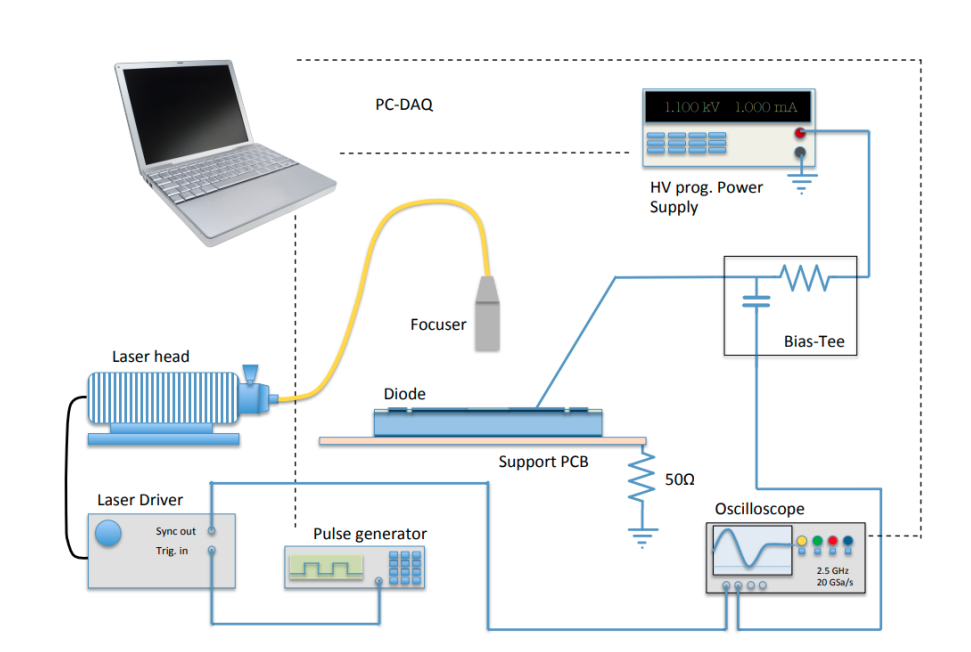
\includegraphics[height=10cm]{fig/imagenLab.png}
\caption{Esquema del montaje experimental para la realización de la práctica de laboratorio.}
\label{fig:laser}
\end{figure} 

El desarrollo de esta práctica requiere que los alumnos se familiaricen con los fundamentos de la física de dispositivos semiconductores comos los diodos. Los alumnos harán cálculos para determinar la forma del campo eléctrico en el interior del diodo, la ``depletion depth'', o el nivel de dopado de los semiconductores. Las medidas principales son la curva ``Voltaje de Bias vs. Intensidad'', y la curva ``Voltaje de Bias vs. carga recolectada''. A partir de dichas curvas los alumnos estimarán las cantidades requeridas.   

\paragraph{Tema 3: La ecuación de Dirac\\\\}

\textbf{Objetivos}

Este capítulo tiene como objetivo presentar la ecuación de Dirac que rige la dinámica de las partículas fermiónicas. En el proceso de derivación de la ecuación se exponen las motivaciones teóricas que llevaron a su desarrollo. Igualmente, el tema profundiza en las implicaciones que la ecuación tiene desde el punto de vista de la aparación de un nuevo tipo de materia, la antimateria, o del surgimiento del espín como una propiedad inherente de las partículas.

\textbf{Resultados del aprendizaje}

\begin{itemize}
    \item Conocer y saber derivar las expresiones de la densidad y la corriente de probabilidad para la ecuación de Schrödinger.
    \item Conocer la derivación de la ecuación de Klein-Gordon a partir de la expresión de la energía relativista y sus expresiones para la densidad y la corriente de probabilidad.
    \item Entender el problema de la energía y densidad de probabilidad negativas para la ecuación de Klein-Gordon. 
    \item Entender la derivación de la ecuación de Dirac como un intento de linearizar la ecuación de Klein-Gordon para evitar el problema de la energía negativa y sus expresiones de densidad y corriente de probabilidad.
    \item Entender el concepto de ``espinor''.
    \item Manejar con destreza la ecuación de Dirac prestando atención al álgebra de conmutación de sus matrices.
    \item Saber cómo derivar soluciones de onda plana para la ecuación de Dirac.
    \item Entender el surgimiento de la antimateria como una nueva especie de partícula que se corresponde con los estados de energía negativos.
    \item Entender el surgimiento del espín como una magnitud que necesariamente ha de añadirse al momento angular orbital para que éste conmute con el Hamiltoniano asociado a la ecuación de Dirac.
    \item Entender el concepto de helicidad.
    \item Saber cómo derivar soluciones de onda plana para la ecuación de Dirac, que sean simultáneamente autoestados de la helicidad.
    \item Entender el concepto de paridad y conjugación de carga y su relación con los espinores de la ecuación de Dirac.
\end{itemize}

\textbf{Contenidos}

El tema comienza con un cálculo de la densidad y corriente de probabilidad, junto con su ecuación de continiudad para la ecuación de Schrödinger. Tras esta derivación se evalua la densidad de probabilidad para una onda plana obteniendo un valor estrictamente positivo. A continuación, se deriva la ecuación de Klein-Gordon, partiendo de la relación energía-momento relativista y haciendo las correspondientes sustituciones de la energía como derivada temporal y del momento como el gradiente espacial. Para esta nueva ecuación se calculan de nuevo la densidad de probabilidad y su corriente. Al evaluar en la ecuación una onda plana se observan dos cosas: existen soluciones de energía tanto positivas como negativas; y la densidad de probabilidad es proporcional a la energía y por lo tanto, no es estrictamente positiva. La interpretación probabilística de la ecuacion de Klein-Gordon es por lo tanto inconsistente. 

Una vez expuesto el problema se incide en el hecho de que la existencia de soluciones con energías negativas parece estar relacionada con la aparación en la ecuación de Klein-Gordon de una derivada temporal de segundo orden. En este punto, se expone cómo Paul Dirac intentó resolver el problema encontrando una ecuación que sólo involucrase derivadas de primer orden. Es evidente que para mantener la consistencia con la relación de energía-momento relativista, al elevar al cuadrado la ecuación linearizada de Dirac debía obtenerse la ecuación de Klein-Gordon. Para que esto sea posible es necesario añadir unos coeficientes a los términos de la ecuación linearizada $\alpha_i$ y $\beta$, que además para reproducir la ecuación de Klein-Gordon han de ser matrices de dimensión 4x4, cumpliendo además reglas de anticonmutación $\{\alpha_i, \alpha_j\}=0$ con $i\neq j$ y $\{\alpha_i, \beta\}=0$. De esta forma queda establecida la ecuación de Dirac como una ecuación de dimensión cuatro y por lo tanto la función de onda ha de contar con cuatro componentes formando lo que se conoce como un ``espinor''.

Una vez la ecuación de Dirac ha sido establecida se estudia su comportamiento desde el punto de vista del momento angular orbital. El conmutador $[H, \vec{L}]$ es calculado para la ecuación de Dirac, poniéndose de manifiesto su no nulidad, lo que implica la imposibilidad de encontrar una base común de autoestados de la energía y el momento angular. Utilizando el resultado del conmutador, se define un operador $\vec{S}$ que hace que el conmutador $[H, \vec{L}+\vec{S}]$ se cancele. Dicho operador involucra a las matrices de Pauli y puede claramente relacionarse con la definición del espín clásico, introducido ad hoc en la teoría de Schrödinger. De esta forma, queda establecido el espín como un momento angular intrínseco que surge de manera natural en el contexto de la ecuación de Dirac.    

A continuación se procede a introducir la ecuación de Dirac en su versión covariante. Para ello, se multiplica a la ecuación de Dirac obtenida previamente por la matriz $\beta$ de modo que se definen las matrices $\gamma^{\mu}$ con $\gamma^0=\beta$ y $\gamma^i=\beta\alpha^i$. Las nuevas matrices cumplen las relaciones de anticonmutación $\{\gamma^i, \gamma^j\}=2g^{\mu\nu}$, en donde $g^{\mu\nu}$ es la métrica de Minkowski. Con esta nueva formulación, y con la definición del espinor adjunto, se procede al cálculo de la densidad y corriente de probabilidad, observándose que la densidad de probabilidad es siempre estrictamente positiva, y que por tanto la ecuación de Dirac proporciona resultados consistentes desde el punto de vista de una interpretación probabilística. Por otro lado, se evaluan en la ecuación de Dirac soluciones de tipo onda plana, para ver qué condiciones tienen que cumplir los espinores para ser soluciones efectivas de la ecuación. Se obtienen un total de cuatro soluciones diferentes, dos con energía positiva y dos con energía negativa.

En este punto, y por simple interés histórico, se repasan algunas interpretaciones de las soluciones de energía negativa, como son la interpretación de Dirac (soluciones de energía negativa como huecos de energía positiva en un mar lleno de electrones de energía negativa) o la interpretación de Feynman-Stückelberg (soluciones de energía negativa como partículas propagándose hacia atrás en el tiempo). Desde un punto de vista experimental, se incide en el descubrimiento del positrón como primera antipartícula por parte de Anderson. Finalmente, se procede con la interpretación moderna en el que las soluciones de energía negativa pueden asimilarse dentro de soluciones de energía negativa con un espinor de una nueva especie, el espinor de antipartícula. De esta forma, resulta posible elegir una base de cuatro soluciones de onda plana en las que todas ellas tienen energía positiva, siendo dos, espinores de partícula, y otros dos espinores de antipartícula. A continuación se procede a la introducción del operador de conjugación de carga que transforma a los espinores de partícula en espinores de antipartícula y viceversa.

Finalmente, el tema introduce el concepto de helicidad como un observable cuyo número cuántico resulta conveniente en el contexto de la ecuación de Dirac. Puesto que el Hamiltoniano de Dirac y la helicidad conmutan, es posible obtener una base de cuatro soluciones que sean autoestados de los dos. La derivación se lleva a cabo resolviendo la ecuación de autovalores asociada a la helicidad sobre los autoestados del Hamiltoniano calculados previamente. Como resultado de este cálculo se obtiene la base de soluciones de la ecuación de Dirac en la que se tienen dos estados de partícula, una con helicidad positiva y otra con helicidad negativa, y dos estados de antipartícula, también con los dos estados de helicidad posibles. Como último elemento del tema se introduce el operador paridad para indicar cómo su autovalor asociado adquiere signo contrario para las partículas y las antipartículas.

\textbf{Actividades}


%\begin{table}[!h]
%\centering
\begin{center}
\begin{tabularx}{\textwidth}{|X|}
\hline\hline
\multicolumn{1}{|c|}{\textbf{Ejercicios de clase}}\\
\hline\hline
Resolución de problemas sencillos relacionados con las propiedades de las matrices $\gamma^{\mu}$ \\
\hline
Resolución de problemas sencillos utilizando las propiedades de la ecuación de Dirac \\
\hline
Cálculo de densidades y corrientes de probabilidad para casos concretos \\
\hline\hline
\multicolumn{1}{|c|}{\textbf{Trabajos de evaluación continua}}\\
\hline\hline
Demostración sobre la mínima dimensión necesaria para las matrices $\alpha^i$ y $\beta$ \\
\hline
Demostración de la invarianza-Lorentz de la ecuación de Dirac \\
\hline
Discusión y presentación en clase del artículo sobre el descubrimiento del positrón \\
\hline
Resolver el átomo de hidrógeno utilizando la ecuación de Dirac\\
\hline\hline
%\end{table}
\end{tabularx}
\end{center}

\paragraph{Tema 4: Interacción por intercambio de partículas\\\\}

\textbf{Objetivos}

Este tema tiene como objetivo principal el tratamiento de las interacciones entre partículas en el contexto de experimentos de colisión. El tema profundiza en los conceptos de tasa de transición y sección eficaz y deriva expresiones para calcularlas a partir de la regla de oro de Fermi, utilizando los conceptos de densidad de estados y elemento de matriz. En segundo lugar, el tema incide en el concepto de interacción como un intercambio de partículas, para acabar explicando los conceptos de partícula virtual, diagramas de Feynman usando el electromagnetismo como ejemplo.

\textbf{Resultados del aprendizaje}

\begin{itemize}
    \item Entender el concepto de tasa de transición y el significado de la regla de oro de Fermi.
    \item Entender el concepto de densidad de estados y ser capaz de derivar su expresión para casos sencillos.
    \item Entender el concepto de elemento de matriz así como de su naturaleza perturbativa.
    \item Entender los parámetros de un experimento de colisión de partículas y derivar a través de ellos el concepto de sección eficaz.
    \item Ser capaces de derivar expresiones para la tasa de transición y sección eficaz para casos sencillos atendiendo únicamente a la densidad de estados.
    \item Entender el concepto de interacción como un intercambio de partículas. 
    \item Entender el concepto de diagrama de Feynman y ser capaces de identificar sus propiedades básicas.
    \item Identificar el Hamiltoniano o potencial de interacción en la electrodinámica cuántica.
    \item Entender y derivar la forma del elemento de matriz para una interacción electromagnética sencilla.
    \item Comprender los elementos básicos de las reglas de Feynman y ser capaces de aplicarlas a casos sencillos.
\end{itemize}

\textbf{Contenidos}

El tema comienza introduciendo el concepto de tasa de transición como la probabilidad por unidad de tiempo de que una partícula efectúe una transición a un estado diferente (por ejemplo, un decaimiento a otras partículas). Se incide en la importancia de esta magnitud como uno de los observables básicos en los experimentos de física de partículas. A continuación se discute la regla de oro de Fermi presentando sus dos componentes fundamentales: la densidad de estados y el Elemento de Matriz. 

El tema continúa profundizando en el concepto de densidad de estados expandiendo su expresión en términos de integrales y deltas de Dirac que hagan explícitas la conservación de la energía y el momento. En este punto, resulta aún más evidente la definición de esta magnitud como el número de estados finales posibles, compatibles con la energía inicial del sistema por unidad de volumen. El siguiente paso consiste en el cálculo de la densidad de estados para una partícula que decae en otras dos partículas. El cálculo parte de un volumen con forma cúbica en el que la aplicación de las condiciones de contorno hace que el momento de las partículas sufra una cuantización. Dentro de ese esquema, se calcula el número de posibles estados $dn$ por unidad de volumen en función del número de posibles valores del momento $|d\vec{p}|$. A continuación se desarrolla este término utilizando el elemento de volumen esférico $|d\vec{p}|=p^2sin(\theta)d\phi d\theta dp$. Asumiendo homegeneidad en el espacio de momento se integran las coordenadas angulares obteniéndose $4\pi p^2dp$. Finalmente, se utiliza la relación energía-momento relativista para relacionar el módulo del momento con la energía para llegar de esta manera a la expresión final. A continuación se utilizan estas expresiones para calcular la dependencia cinemática del elemento de matriz para el caso en el que una partícula decae en el sistema de referencia de su centro de masas obteniendo. 

Tras la definición de la tasa de transición, se presenta el esquema tradicional de los experimentos de colisión en el que dos haces de partículas colisionan entre sí. En este contexto, se define el concepto de flujo asociado a un haz, y se introduce la probabilidad por unidad de tiempo y partícula de que se produzca una interacción. En este contexto se define la sección eficaz de interacción, aportando su interpretación geométrica y exponiendo también el concepto de sección eficaz diferencial. Una vez halladas las expresiones de la sección eficaz se calcula para casos concretos como la colisión de dos partículas en el sistema de referencia del centro de masas y en el sistema de referencia de laboratorio en el que una de las partículas está en reposo.  

Una vez analizadas las propiedades de la densidad de estados, el tema continúa desarrollando el elemento de matriz como la parte de la regla de oro de Fermi que contiene la dinámica de la interacción. En primer lugar, se parte de la expresión perturbativa del elemento de matriz y se desarrolla el concepto de intercambio de partículas. A tal efecto, se modeliza el proceso de interacción como compuesto por un estado inicial en el que están presentes las dos partículas que interaccionan, $a$ y $b$, un estado intermedio en el que una de las partículas iniciales, $a$, decae en otras dos, $a\rightarrow c + x$, siendo $x$ absorbida por la partícula $b$ y transformándose en $d$, $b + x\rightarrow d$, y un estado final en el quedan como resultantes $c$ y $d$. En este esquema, en el que se han identificados los estados iniciales, finales e intermedio, es posible calcular el elemento de matriz introduciendo el potencial de interacción $V$. En este punto se pone de manifiesto la arbitrariedad introducida en el planteamiento anterior al haber atribuido a la partícula $a$ el papel de emisor y a la partícula $b$ el papel de receptor. Para resolver la arbitrariedad, se suma al elemento de matriz, la contribución correspondiente a la inversión de papeles entre $a$ y $b$, obteniéndose así una expresión final para el elemento de matriz $T_{ab\rightarrow cd}$. Llegados a este punto, se define un elemento de matriz invariante Lorentz, $M_{ab\rightarrow cd}$, utilizando funciones de onda normalizadas a dos veces el valor de la energía. De manera trivial, $M_{ab\rightarrow cd}$ y $T_{ab\rightarrow cd}$ se relacionan a través de los productos de las energías de las partículas involucradas, y por lo tanto, puede utilizarse la expresión obtenida para $T_{ab\rightarrow cd}$ para derivar la expresión de $M_{ab\rightarrow cd}$, que ahora tendrá una expresión manifiestamente invariante Lorentz: $M_{ab\rightarrow cd}=<\Psi_c|V_{int}|\Psi_a>\frac{1}{q^2-m_{x}^2}<\Psi_d|V_{int}|\Psi_b>$. De esta manera, se establece una identificación entre el elemento de matriz y los llamados diagramas de Feynman. Y en este contexto se introduce también el concepto de partícula virtual para hacer referencia a aquellas partículas que propagan la fuerza y cuyos estados no se corresponden con sus estados de masa. 

El siguiente desarrollo del tema persigue la aplicación de estos conceptos al caso particular de la fuerza electromagnética. Para ello, se repasa el concepto de teoría Gauge, que en el caso del electromagnetismo, derivará de una transformación de fase local del tipo $\Psi' = e^{-i\alpha(x)}\Psi$ que se corresponde con un grupo de tipo U(1). Dicha transformación propicia la aparación de un término $-q_e\gamma^\mu A_{\nu}\Psi$ en la ecuación de Dirac, pudiéndose identificar el potencial de interacción con $V_{int}=q_e\gamma^0\gamma^\mu A_\mu$, siendo $A_\mu$ el cuadripotencial vector. Introduciendo este resultado en la expresión del elemento de matriz $M_{ab\rightarrow cd}$, puede desarrollarse el término como  $M_{ab\rightarrow cd}=<\Psi_c|q_e\gamma^0\gamma^\mu|\Psi_a>\frac{A_\mu A_\nu}{q^2-m_{x}^2}<\Psi_d|q_e\gamma^0\gamma^\nu|\Psi_b>$. Tras las correspondientes integraciones de momento y sustituyendo las funciones de onda por sus espinores, y en el caso del cuadripotencial vector, sumando a todos los posibles estados de polarización $\epsilon_\nu^\lambda$, se obtiene $M_{ab\rightarrow cd}=<\Psi_c|q_e\gamma^0\gamma^\mu|\Psi_a>\frac{\sum_{\lambda}\epsilon_\mu^\lambda\epsilon_\nu^\lambda}{q^2-m_{x}^2}<\Psi_d|q\gamma^0\gamma^\nu|\Psi_b>=[\bar{u_c}q_e\gamma^\mu u_a]\frac{-g_{\mu\nu}}{q^2}[\bar{u_d}q_e\gamma^\nu u_b]$. Finalmente se definen las cuadricorrientes $j_{ac}^\mu=\bar{u_c}\gamma^\mu u_a$ y $j_{bd}^\nu=\bar{u_d}\gamma^\nu u_b$, de manera que el elemento de matriz puede escribirse fácilmente como: $M_{ab\rightarrow cd}=q_e^2\frac{j_{ac}j_{bd}}{q^2}$. 

Finalmente, el tema generaliza el desarrollo para enumerar las reglas de Feynman para el electromagnetismo en el que las líneas entrantes y salientes de los diagramas aportan sus espinores o espinores adjuntos respectivamente, los vértices aportan el término $iq_e\gamma^{\mu}$ y los fotones de intercambio el término $-i\frac{g_{\mu\nu}}{q^2}$.

\textbf{Actividades}


%\begin{table}[!h]
%\centering
\begin{center}
\begin{tabularx}{\textwidth}{|X|}
\hline\hline
\multicolumn{1}{|c|}{\textbf{Ejercicios de clase}}\\
\hline\hline
Ejercicios acerca de la validez de diagramas de Feynman propuestos \\
\hline
Dibujar diagramas de Feynman asociados a procesos sencillos \\
\hline 
Cálculo de cantidades relevantes en procesos de scattering \\
\hline\hline
\multicolumn{1}{|c|}{\textbf{Trabajos de evaluación continua}}\\
\hline\hline
Demostrar el origen del término de interacción electromagnético aplicando la transformación local gauge U(1) y observando su efecto en la Lagrangiana de Dirac \\
\hline
Demostrar cuál es el número de estados posibles de polarización de un fotón \\
\hline
Demostrar que la suma de los vectores de polarización de los fotones es igual a menos el tensor métrico de Minkowski \\
\hline\hline
%\end{table}
\end{tabularx}
\end{center}


\paragraph{Capítulo 5: Aniquilación electrón-positrón\\\\}

\textbf{Objetivos}

Este tema tiene como objetivo el cálculo detallado de la sección eficaz y de la sección eficaz diferencial del proceso de aniquilación electrón-positrón. En el cálculo del elemento de matriz correspondiente se tendrán en cuenta todos los posibles estados de helicidad de las partículas entrantes y salientes, prestando atención a las diferencias entre diferentes combinaciones. El tema introduce finalmente el concepto de quiralidad como límite de la helicidad para partículas sin masa.   

\textbf{Resultados del aprendizaje}

\begin{itemize}
    \item Entender las diferencias entre un haz polarizado de fermiones (helicidad única bien determinada) o un haz no polarizado (mezcla de helicidades).
    \item Ser capaz de aplicar las reglas de Feynman para el caso de la aniquilación electrón-positrón utilizando los espinores autoestados de la helicidad.
    \item Entender que las contribuciones a la sección diferencial de este proceso dependen fuertemente de las helicidades de las partículas entrantes y salientes. 
    \item Entender el concepto de quiralidad.
    \item Comprender y saber realizar cálculos sencillos con los operadores de proyección quiral.
\end{itemize}

\textbf{Contenidos}

Este tema comienza describiendo las condiciones de helicidad en las que se suelen produciar la mayor parte de los experimentos de colisión de fermiones. Salvo en algunos experimentos específicos donde los haces de fermiones son filtrados y preparados convenientemente, su composición de helicidades suele contener una mezcla equiprobable de estados positivos y negativos. La sección eficaz total del proceso vendrá dada por la suma de las secciones eficaces de interacción asociadas a cada combinación de helicidad entrante, pero también a cada combinación de helicidad saliente. Por lo tanto resulta necesario calcular los elementos de matriz $M_{XY\rightarrow X'Y'}$ en donde X, Y, X' e Y' hacen referencia a las helicidades de las dos partículas entrantes y salientes respectivamente.

En el resto del capítulo se llevan a cabo estos cálculos aplicando las reglas de Feynman con los espinores autoestados de la helicidad correspondientes. Para simplificar la tarea, se asumirá en todo momento que las partículas se encuentran en el límite relativista en el que $m\approx 0$. El cálculo de las corrientes para cada caso y su producto refleja cómo aquellas combinaciones en las que las partículas entrantes o salientes tienen la misma helicidad entre sí, el elemento de matriz se anula. Esto permite identificar los diferentes casos simplemente a través del estado de helicidad de la partícula entrante o saliente, ya que la correspondiente antipartícula ha de tener helicidad opuesta para que el elemento de matriz no sea nulo. 

En estas condiciones se calculan las secciones eficaces diferenciales para los cuatro casos posibles $M_{R\rightarrow R}$, $M_{R\rightarrow L}$, $M_{L\rightarrow R}$, $M_{L\rightarrow L}$, en donde en este caso la helicidad hace referencia únicamente a la partícula (en oposición a la antipartícula). Los resultados arrojan el siguiente resultado: las secciones eficaces diferenciales de los casos con igual helicidad, RR o LL, contribuyen con un término $(1 + cos(\theta))^2$ y por lo tanto tienen mayor probabilidad de que la partícula (antipartícula) saliente vaya en una dirección parecida a la de la partícula (antipartícula) incidente. Por el contrario los casos RL y LR contribuyen con un término $(1 - cos(\theta))^2$, haciendo que la probabilidad sea mayor de que la partícula (antipartícula) saliente vaya en la dirección de la antipartícula (partícula) entrante. Finalmente, se comparan estos resultados con las medidas de algunos experimentos del siglo XX que estudiaron el proceso en detalle.

El tema continúa introduciendo el concepto de quiralidad. La quiralidad es un operador que coincide con la helicidad en el caso de partículas no masivas. En ese límite los autoestados de helicidad son también autoestados de la quirilidad. Fuera de ese límite los autoestados de helicidad positiva tienen una componente no nula de los dos estados de quiralidad. Resulta práctico para obtener dicha componente definir los operadores de proyección quiral $P_R$ y $P_L$ que proyectan un estado cualquiera sobre el espacio de quiralidad ``left-handed'' y ``right-handed'' respectivamente. Las propiedades observadas anteriormente acerca del valor de los elementos de matriz puede ponerse en términos de la quiralidad. Esto resulta particularmente relevante, ya que la fuerza débil que se explicará a continuación tiene un comportamiento muy diferente desde el punto de vista de la quiralidad.

\textbf{Actividades}

%\begin{table}[!h]
%\centering
\begin{center}
\begin{tabularx}{\textwidth}{|X|}
\hline\hline
\multicolumn{1}{|c|}{\textbf{Ejercicios de clase}}\\
\hline\hline
Ejercicios sobre el cálculo de elementos de matriz para fermiones polarizados \\
\hline
Ejercicios acerca de las propiedades de los operadores de proyección quiral \\
\hline\hline
\multicolumn{1}{|c|}{\textbf{Trabajos de evaluación continua}}\\
\hline\hline
Relacionar las reglas de selección de helicidad con el spin de las partículas \\
\hline\hline
%\end{table}
\end{tabularx}
\end{center}

\paragraph{Tema 6: La interacción electrodébil\\\\}

\textbf{Objetivos}

Este tema tiene como objetivo proporcionar una descripción de los fundamentos básicos de la fuerza débil. El punto de partida será el análisis de las propiedades de paridad de la fuerza electromagnética así como el experimento de Madame Wu que demostró que existían interacciones que violaban dicha paridad. Posteriormente se derivarán reglas de Feynman que sean capaces de violar la paridad y se identificarán éstas con la fuerza débil. Finalmente, el tema construye la teoría débil a través de un principio de invarianza Gauge y proporciona el mecanismo de unificación de las fuerzas electromagnética y débil.

\textbf{Resultados de aprendizaje}

\begin{itemize}
    \item Entender el concepto de paridad y el significado de que un proceso físico no la conserve.
    \item Comprender la relevancia del experimento de Madame Wu.
    \item Ser capaces de derivar cuadri-corrientes con capacidad para violar la paridad del sistema y relacionarlas con las propiedades quirales de las partículas.
    \item Comprender la relevancia del decaimiento del pion cargado.
    \item Conocer y entender el significado de la constante de Fermi y de los conceptos de hipercarga débil e isospin débil.
    \item Entender la interacción débil a través de un principio de invarianza Gauge.
    \item Comprender el principio de unificación de la fuerza electromagnética y débil.
    \item Entender el significado del ángulo de ``mixing'' $\theta$.
    \item Ser capaces de aplicar las reglas de Feynman para la teoría electrodébil.
    \item Entender el concepto de resonancia y de cómo medir su anchura con datos de un aceleradon hadrónico.
\end{itemize}

\textbf{Contenidos}

El tema comienza analizando la invarianza de los elementos de matriz $M$ de la electrodinámica cuántica cuando sobre sus espinores se ejecuta una transformación de paridad. A continuación, se introduce el experimento de Madame Wu en el que a través del estudio de decaimientos de núcleos de Cobalto se observó una violación de la paridad, sugiriendo que el origen de la interacción que había provocado los decaimientos era diferente a la electromagnética. En este punto, se introducen los conceptos de bilineales covariantes como escalares, pseudoescalares, axial, axial-vector, etc; y se comprueba cómo el uso de reglas de Feynman con vértices que contengan una combinación lineal de un bilineal axial y axial-vector $(\gamma^\mu + a\gamma^5\gamma^\mu)$ proporciona una violación de paridad, desde el punto de vista de que el elemento de matriz es diferente cuando se transforman los espinores a través del operador de paridad. Se establece que los experimentos determinan que la violación de paridad ha de ser máxima, lo cuál hace coincidir la forma de los vértices con los operadores de proyección quiral para partículas y antipartículas respectivamente. Finalmente se identifican estas propiedades con la fuerza débil, mostrándose cómo este tipo de interacción puede verse como una interacción que sólo es efectiva con la parte ``left-handed'' (``right-handed'') de las (anti)partículas. A continuación se analiza uno de los casos más paradigmáticos en el que este efecto se manifiesta ampliamente: el decaimiento del pion cargado. Este proceso se analizará en detalle, estimando cuál es la fracción de quiralidad ``left-handed'' tienen los electrones y muones de helicidad positiva y negativa respectivamente. En este punto, se muestran las reglas de Feynman para este tipo de interacción prestando atención a la constante de la fuerza débil.

Una vez analizada esta fenomenología, se procede a introducir la interacción débil como una teoría Gauge, en la que se establecen transformaciones de simetría SU(2)$_L$ y se construyen los nuevos espinores asociados a la fuerza débil como elementos de un espacio de 2 dimensiones que se corresponden con la fracción de leptón cargado y neutrino de dicho elemento. La aplicación de transformaciones de fase locales en este espacio de dos dimensiones genera la aparición de 3 nuevas partículas de interacción $W_1$, $W_2$ y $W_3$, moduladas por las tres matrices de Pauli propias de la representación SU(2). Combinaciones de los bosones $W_1$ y $W_2$, gracias a las propiedades de las matrices de Pauli, pueden identificarse con los bosones $W^+$ y $W^-$ que se observan en las interacciones débiles que conllevan corrientes cargadas. Sin embargo, la teoría Gauge predice un nuevo bosón $W_3$ cuya existencia estaba ya postulada ya que los procesos de producción de pares $W^+W^-$ con las partículas conocidas hasta la época violaban el principio de unitariedad, siendo necesaria la adición de algún diagrama adicional que mantuviese al elemento de matriz acotado.

El bosón $W_3$ podría ser identificado con el bosón $Z$, sin embargo, debido al mecanismo de ruptura de simetría por el que los bosones adquieren masa (ver~\ref{bosonhiggs}) puede inferirse que en realidad el bosón $Z$, y de la misma forma el fotón $A$, son en realidad combinaciones lineales del estado $W_3$ y de un nuevo bosón $B$. La fracción que determina el grado de combinación se da como un ángulo, el ángulo de ``mixing''. De esta forma, la fuerza electromagnética y la fuerza débil quedan unificadas como la manifestación de un mismo fenómeno. A continuación, y utilizando el ángulo de ``mixing'' pueden relacionarse la constante de fuerza electromagnética y la débil. Igualmente, usando las propiedades de los bosones $W_3$ y $B$ pueden derivarse las reglas de Feynman para el bosón Z. 

Finalmente, en este tema se realiza una práctica computacional centrada en la medida de las propiedades del bosón Z utilizando datos del experimento CMS y que se describen a continuación. 

\textbf{Actividades}


%\begin{table}[!h]
%\centering

\begin{center}
\begin{tabularx}{\textwidth}{|X|}
\hline\hline
\multicolumn{1}{|c|}{\textbf{Ejercicios de clase}}\\
\hline\hline
Ejercicio relacionado con el experimento de Madame Wu \\
\hline
Ejercicio relacionados con la fracción de quiralidad en estados de helicidad puros \\
\hline\hline
\multicolumn{1}{|c|}{\textbf{Trabajos de evaluación continua}}\\
\hline\hline
Obtener los estados de polarización de los bosones masivos \\
\hline\hline
\multicolumn{1}{|c|}{\textbf{Actividad en grupo}}\\
\hline\hline
El experimento de Madame Wu. Competición usando \emph{Socrative - Space Race}\\
\hline\hline
\multicolumn{1}{|c|}{\textbf{Práctica de ordenador}}\\
\hline\hline
Medida de la anchura del bosón Z con datos de CMS\\
\hline\hline
%\end{table}
\end{tabularx}
\end{center}

\textbf{Actividad en grupo}

La actividad en grupo tiene su origen en el empleo de la técnica de ``Flipped classroom'' en la que se intercambia la parte de transmisión de conocimiento, tradicionalmente hecha en el aula durante la clase magistral, al trabajo autónomo del alumno, sustituyendo el tiempo en clase por alguna actividad de refuerzo y aplicación de los conocimientos. En este caso concreto, la propuesta está relacionada con el experimento de Madame Wu. Los alumnos reciben por parte del profesor, el artículo de Madame Wu sobre la violación de paridad, así como otros recursos públicos que explican el experimento. Posteriormente los alumnos se organizan en equipos y se dedica un espacio de aproximadamente 20 minutos para que dichos alumnos, trabajando en grupo, resuelven una prueba con preguntas sobre el experimento de Madame Wu. La plataforma utilizada es Socrative\footnote{\url{www.socrative.com}}, en su modalidad de ``Space Race'', de manera que los diferentes equipos pueden ver de forma interactiva su puntuación en un formato que simula una carrera. 

\textbf{Práctica de ordenador}

La práctica de ordenador constituye una introducción al análisis de datos en los grandes detectores de partículas como es el detector CMS. El título de la práctica es ``Medida de la anchura del bosón Z con datos de CMS''. El objetivo fundamental de la práctica es que los alumnos se familiaricen con las herramientas de análisis de datos de física de partículas, como ROOT\footnote{\url{http://root.cern.ch}}, que repasen los conceptos de cómo funcionan los grandes detectores de partículas y que profundicen en el concepto de resonancia en el contexto de física de partículas y más concretamente en la del bosón Z.

Esta práctica se desarrolla en una aplicación tecnológica conocida como ``Jupyter notebook''\footnote{\url{http://jupyter.org}} que permite acceder a través del navegador, a terminales con un entorno completo de programas y datos previamente cargados. En este caso concreto, el alumno se encontrára con un entorno del lenguaje de programación Python con las librerías de la herramienta de análisis ROOT. El alumno también tendrá acceso a datos de colisiones recogidos por el experimento CMS y filtrados para contener sucesos con muones. En el transcurso de la práctica los alumnos tendrán que determinar cómo seleccionar los sucesos atendiendo a los diferentes indicadores de calidad de los objetos presentes en ellos. El objetivo final es el de obtener una gráfica aceptable de la masa invariante de los dos muones presentes en el suceso, en la que se observe la resonancia del bosón Z. Una vez obtenida esta gráfica se realizará un ajuste de dicha resonancia para estimar su anchura.




\paragraph{Capítulo 7: Introducción a la interacción fuerte\\\\}

\textbf{Objetivos}

El objetivo principal de este tema consiste en dar una visión general y breve acerca de la interacción fuerte. Para ello se introduce brevemente el modelo de quarks que derivó en la existencia de una carga fuerte, el color, con tres valores posibles. En virtud de esta carga, se utiliza el principio de invarianza Gauge dando lugar a los 8 gluones que median la interacción fuerte. A continuación se discuten conceptos como el confinamiento de color y se estudia cómo construir funciones de onda adecuadas para los posibles mesones y bariones. Finalmente se detallan las reglas de Feynman para la interacción fuerte. 

\textbf{Resultados del aprendizaje}

\begin{itemize}
    \item Entender el concepto de color como la carga asociada a la fuerza fuerte.
    \item Comprender el modelo de quarks y su relación con los mesones y bariones observados en la naturaleza.
    \item Entender el concepto de confinamiento de color.
    \item Entender los conceptos de isospin fuerte e hipercarga fuerte.
    \item Ser capaces de derivar funciones de onda para mesones y bariones sencillos; y para gluones
    \item Entender el concepto de hadronización y de jet.
    \item Entender la estructura de las reglas de Feynman para la fuerza fuerte.
    
\end{itemize}

\textbf{Contenidos}

El tema comienza exponiendo el concepto de color como la carga asociada a la fuerza fuerte y por lo tanto como una propiedad de los quarks. En base a los tres posibles valores del color, se aplica el principio de invarianza Gauge, proponiendo funciones de onda en un espacio de 3 dimensiones e imponiendo rotaciones en este espacio de acuerdo con las transformaciones del grupo SU(3). Dadas las características del grupo SU(3) la imposición de la invarianza Lagrangiana antes estas transformaciones da lugar a la aparación de 8 nuevos bosones, modulados por las matrices de Gell-Mann. A continuación se introducen también los conceptos de isospin fuerte e hipercarga fuerte.

Una vez introducidos los principios de la fuerza fuerte se profundiza en el concepto de confinamiento de color, según el cuál, los quarks sólo dan lugar a estados ligados estables cuando éstos tienen un color global neutro. Esta observación experimental impone condiciones a la manera en la que se construyen las funciones de onda de los mesones (combinaciones de 2 quarks) y bariones (combinaciones de 3 quarks), así como condiciones al número de quarks que pueden combinarse para formar estados ligados. Ejemplos acerca de la construcción de funciones de onda de mesones y bariones son estudiados en este punto. A continuación, se estudian las funciones de onda de los gluones. Puesto que los gluones no son estables, su color neto no ha de ser neutro, dando lugar a 8 posibles gluones con combinaciones de color y anticolor. 

Posteriormente se estudian las interacciones de los gluones consigo mismos y se presenta el concepto de hadronización. Dos quarks producidos en libertad interaccionan a través de redes de gluones que acaban dando lugar a nuevos quarks que se combinan con los iniciales para producir estados neutros de color. Este proceso es conocido como hadronización y su huella en los detectores de partículas es lo que se conoce como un ``jet''. Finalmente se explican los experimentos de producción de jets en interacciones electromagnéticas como una manera de confirmar la multiplicidad debida al color así como las cargas fraccionales de los quarks. Para concluir, el tema presenta de forma somera las reglas de Feynman para el caso de la fuerza fuerte incluyendo la evolución de los factores de color y sus sumas. 


\textbf{Actividades}
%\begin{table}[!h]
%\centering

\begin{center}
\begin{tabularx}{\textwidth}{|X|}
\hline\hline
\multicolumn{1}{|c|}{\textbf{Ejercicios de clase}}\\
\hline\hline
Cálculos sencillos de factores de color con las matrices de Gell-Mann\\
\hline\hline
\multicolumn{1}{|c|}{\textbf{Trabajos de evaluación continua}}\\
\hline\hline
Resumen y breve presentación del resultado sobre pentaquarks de LHC-b en 2015 \\
\hline\hline
%\end{table}
\end{tabularx}
\end{center}


\paragraph{Capítulo 8: El bosón de Higgs\\\\}\label{bosonhiggs}

\textbf{Objetivos}

Este tema tiene como objetivo presentar una introducción al mecanismo de ruptura de simetría propuesto por Brout, Englert y Higgs, por el cuál las partículas del Modelo Estándar adquieren masa a través de una interacción con un bosón escalar llamado Bosón de Higgs. 

\textbf{Resultados del aprendizaje}

\begin{itemize}
    \item Entender el problema que los bosones $W^{+}$, $W^{-}$ y $Z$ presentaban por el hecho de ser masivos, al provocar los términos de masa que la Lagrangiana no fuese invariante ante las transformaciones Gauge correspondientes.
    \item Entender el Mecanismo de Ruptura de Simetría a través de la introducción en la Lagrangiana de un campo escalar con un potencial del tipo $V(\Phi)=\mu^2\Phi^2/2 + \lambda\Phi^4/4$.
    \item Entender que el desarrollo del nuevo campo en torno a su mínimo da lugar a un término de masa en la lagrangiana.
    \item Entender el concepto de bosón de Goldstone.
    \item Entender cómo aplicar este concepto al caso de una teoría Gauge U(1).
    \item Entender cómo aplicar este concepto al Modelo Estándar con una teoría Gauge U(1)xSU(2)$_L$: aparición de los bosones $A$, $W^{+}$, $W^{-}$ y $Z$.
    \item Entender de forma breve el mecanismo por el que los fermiones adquieren masa incluyendo el mecanismo de ``seesaw'' y el concepto de masa de Majorana.
\end{itemize}

\textbf{Contenidos}

Este capítulo comienza describiendo los problemas que surgen en la Lagrangiana de un supuesto Modelo Estándar con bosones de intercambio masivos. En efecto, la aparición de dichos bosones hace que la Lagrangiana no sea invariante ante transformaciones Gauge U(1) y SU(2)$_L$. Con objeto de resolver este problema, Brout, Englert y Higgs, desarrollaron un mecanismo basado en la introducción de un nuevo campo escalar $\Phi$ dotado de un potencial con la estructura: $V(\Phi)=\mu^2\Phi^2/2 + \lambda\Phi^4/4$. En el caso de un campo escalar de una dimensión, el mínimo de potencial no se encuentra para el valor nulo del campo, sino para dos valores $\Phi = \pm v$ distintos de 0. La naturaleza romperá la simetría escogiendo uno de los dos, de manera, que se puede redefinir el campo en torno a dicho mínimo de la forma $\Phi = v + \eta(x)$. Escribiendo la Lagrangiana en términos de este nuevo campo $\eta$ es posible comprobar que este mecanismo hace surgir un término de masa para el nuevo campo $\eta$. 

A continuación se desarrolla este concepto en términos de una teoría gauge U(1). Para ello, se define un campo análogo al anterior pero en el dominio complejo $\Phi = \Phi_1 + i \Phi_2$ y de nuevo un potencial de tipo $V(\Phi)=\mu^2\Phi^2/2 + \lambda\Phi^4/4$. El mínimo del potencial es un conjunto infinito de puntos que cumplen que $\Phi_!^2+\Phi_2^2 = v^2$. En estas condiciones se redefinen nuevos campos en torno al mínimo, elegido sin pérdida de generalidad como un número real en $\Phi=v$. Los nuevos campos son: $\Phi = v + \eta(x) + i \xi(x)$. En este punto, se exige que la Lagrangiana asociada a estos campos, que incluye el término cinemático y el de potencial, sea invariante bajo transformaciones Gauge $\Phi'=e^{-i\alpha(x)}\Phi$, dando lugar a la aparición de un nuevo bosón Gauge $B$. El desarrollo de la Lagrangiana completa en términos de $\eta$ y $\xi$, eligiendo los Gauge adecuados para el bosón $B$ da lugar a una Lagrangiana en la que aparecen los términos cinéticos de $\eta(x)$ y el bosón $B$ ambos con un término de masa, y los correspondientes términos de interacción entre ellos y entre sí mismos. 

Una vez explicado el mecanismo para el caso sencillo de una teoría U(1), el concepto se aplica al Modelo Estándar. Puesto que en este modelo hay un total de 3 bosones masivos, es necesario ampliar la dimensión del campo $\Phi$, por lo que se escoge como un doblete de dos campos complejos $\Phi=(\Phi_1, \Phi_2)$. Finalmente, el procedimiento llevado a cabo en detalle para el caso de U(1) se repite de forma superficial para el caso U(1)xSU(2)$_L$, mostrando cómo al final, en este contexto, es posible redefinir los bosones de intercambio para que sus términos de masa aparezcan en la Lagrangiana. 

La parte final del capítulo se dedica a describir de manera muy superficial cómo el mecanismo de Brout-Englert-Higgs permite también que los fermiones adquieran masa a través del mecanismo seesaw. Finalmente se discuten brevemente conceptos como la masa de Majorana y las masas de los neutrinos.


\textbf{Actividades}
%\begin{table}[!h]
%\centering
\begin{center}
\begin{tabularx}{\textwidth}{|X|}
\hline\hline
\multicolumn{1}{|c|}{\textbf{Trabajos de evaluación continua}}\\
\hline\hline
Resumen y breve presentación del descubrimiento del bosón de Higgs por parte de CMS y ATLAS en el año 2012 \\
\hline\hline
%\end{table}
\end{tabularx}
\end{center}




